% This is file JFM2esam.tex
% first release v1.0, 20th October 1996
%       release v1.01, 29th October 1996
%       release v1.1, 25th June 1997
%       release v2.0, 27th July 2004
%   (based on JFMsampl.tex v1.3 for LaTeX2.09)
% Copyright (C) 1996, 1997 Cambridge University Press

\NeedsTeXFormat{LaTeX2e}

\documentclass{jfm}
%\documentclass[referee]{jfm} %for double spaced output for submission


\usepackage{graphicx}
\usepackage{natbib}

\usepackage{color}
\usepackage{soul}
\usepackage{booktabs}
\pdfoptionpdfminorversion 4

% \pdfcompresslevel0

% See if the author has AMS Euler fonts installed: If they have, attempt2
% to use the 'upmath' package to provide upright math.
\ifCUPmtlplainloaded \else
  \checkfont{eurm10}
  \iffontfound
    \IfFileExists{upmath.sty}
      {\typeout{^^JFound AMS Euler Roman fonts on the system,
                   using the 'upmath' package.^^J}%
       \usepackage{upmath}}
      {\typeout{^^JFound AMS Euler Roman fonts on the system, but you
                   dont seem to have the}%
       \typeout{'upmath' package installed. JFM.cls can take advantage
                 of these fonts,^^Jif you use 'upmath' package.^^J}%
       \providecommand\upi{\pi}%
      }
  \else
    \providecommand\upi{\pi}%
  \fi
\fi

% See if the author has AMS symbol fonts installed: If they have, attempt
% to use the 'amssymb' package to provide the AMS symbol characters.

\ifCUPmtlplainloaded \else
  \checkfont{msam10}
  \iffontfound
    \IfFileExists{amssymb.sty}
      {\typeout{^^JFound AMS Symbol fonts on the system, using the
                'amssymb' package.^^J}%
       \usepackage{amssymb}%
       \let\le=\leqslant  \let\leq=\leqslant
       \let\ge=\geqslant  \let\geq=\geqslant
      }{}
  \fi
\fi

% See if the author has the AMS 'amsbsy' package installed: If they have,
% use it to provide better bold math support (with \boldsymbol).

\ifCUPmtlplainloaded \else
  \IfFileExists{amsbsy.sty}
    {\typeout{^^JFound the 'amsbsy' package on the system, using it.^^J}%
     \usepackage{amsbsy}}
    {\providecommand\boldsymbol[1]{\mbox{\boldmath $##1$}}}
\fi

%%% Example macros (some are not used in this sample file) %%%

% For units of measure
\newcommand\dynpercm{\nobreak\mbox{$\;$dyn\,cm$^{-1}$}}
\newcommand\cmpermin{\nobreak\mbox{$\;$cm\,min$^{-1}$}}

% Various bold symbols
\providecommand\bnabla{\boldsymbol{\nabla}}
\providecommand\bcdot{\boldsymbol{\cdot}}
\newcommand\biS{\boldsymbol{S}}
\newcommand\etb{\boldsymbol{\eta}}

% For multiletter symbols
\newcommand\Real{\mbox{Re}} % cf plain TeX's \Re and Reynolds number
\newcommand\Imag{\mbox{Im}} % cf plain TeX's \Im
\newcommand\Rey{\mbox{\textit{Re}}}  % Reynolds number
\newcommand\Pran{\mbox{\textit{Pr}}} % Prandtl number, cf TeX's \Pr product
\newcommand\Pen{\mbox{\textit{Pe}}}  % Peclet number
\newcommand\Ai{\mbox{Ai}}            % Airy function
\newcommand\Bi{\mbox{Bi}}            % Airy function

% For sans serif characters:
% The following macros are setup in JFM.cls for sans-serif fonts in text
% and math.  If you use these macros in your article, the required fonts
% will be substitued when you article is typeset by the typesetter.
%
% \textsfi, \mathsfi   : sans-serif slanted
% \textsfb, \mathsfb   : sans-serif bold
% \textsfbi, \mathsfbi : sans-serif bold slanted (doesnt exist in CM fonts)
%
% For san-serif roman use \textsf and \mathsf as normal.
%
\newcommand\ssC{\mathsf{C}}    % for sans serif C
\newcommand\sfsP{\mathsfi{P}}  % for sans serif sloping P
\newcommand\slsQ{\mathsfbi{Q}} % for sans serif bold-sloping Q

% Hat position
\newcommand\hatp{\skew3\hat{p}}      % p with hat
\newcommand\hatR{\skew3\hat{R}}      % R with hat
\newcommand\hatRR{\skew3\hat{\hatR}} % R with 2 hats
\newcommand\doubletildesigma{\skew2\tilde{\skew2\tilde{\Sigma}}}
%       italic Sigma with double tilde

% array strut to make delimiters come out right size both ends
\newsavebox{\astrutbox}
\sbox{\astrutbox}{\rule[-5pt]{0pt}{20pt}}
\newcommand{\astrut}{\usebox{\astrutbox}}

\newcommand\GaPQ{\ensuremath{G_a(P,Q)}}
\newcommand\GsPQ{\ensuremath{G_s(P,Q)}}
\newcommand\p{\ensuremath{\partial}}
\newcommand\tti{\ensuremath{\rightarrow\infty}}
\newcommand\kgd{\ensuremath{k\gamma d}}
\newcommand\shalf{\ensuremath{{\scriptstyle\frac{1}{2}}}}
\newcommand\sh{\ensuremath{^{\shalf}}}
\newcommand\smh{\ensuremath{^{-\shalf}}}
\newcommand\squart{\ensuremath{{\textstyle\frac{1}{4}}}}
\newcommand\thalf{\ensuremath{{\textstyle\frac{1}{2}}}}
\newcommand\Gat{\ensuremath{\widetilde{G_a}}}
\newcommand\ttz{\ensuremath{\rightarrow 0}}
\newcommand\ndq{\ensuremath{\frac{\mbox{$\partial$}}{\mbox{$\partial$} n_q}}}
\newcommand\sumjm{\ensuremath{\sum_{j=1}^{M}}}
\newcommand\pvi{\ensuremath{\int_0^{\infty}%
  \mskip \ifCUPmtlplainloaded -30mu\else -33mu\fi -\quad}}

\newcommand\etal{\mbox{\textit{et al.}}}
\newcommand\etc{etc.\ }
\newcommand\eg{e.g.\ }


\newcommand{\uu}{\textbf{u}}
\newcommand{\xx}{\textbf{x}}
\newcommand{\kk}{\textbf{k}}
\newcommand{\JJ}{\textbf{J}}
\newcommand{\rr}{\textbf{r}}
\newcommand{\ff}{\textbf{f}}
\newcommand{\FF}{\textbf{F}}
\newcommand{\baa}{\textbf{a}}
\newcommand{\bb}{\textbf{b}}
\newcommand{\NN}{\textbf{N}}


\newcommand{\eps}{\varepsilon}


\newcommand{\ErtelPV}{\mathcal{Q}}

\newcommand{\fdiss}{f_{\mbox{\scriptsize diss}}}

\newcommand{\D}{\mbox{D}}

\newcommand{\eez}{\boldsymbol{e_z}}
\newcommand{\scalarprod}[2]{\big( #1 \, , \ #2 \big)_{\kk}}

\newcommand{\mean}[1]{\langle #1 \rangle}

\newcommand{\meane}[1]{\langle #1 \rangle}
% \newcommand{\meane}[1]{{\langle #1 \rangle_{\hspace{-0.4mm}e}}}

\newcommand{\meanx}[1]{{\langle #1 \rangle_{\hspace{-0.4mm}\mbox{\scriptsize$\xx$}}}}

\newcommand{\meant}[1]{{\langle #1 \rangle_{\hspace{-0.4mm}\theta}}}

\newcommand{\means}[1]{{\langle #1 \rangle_{\hspace{-0.4mm}s}}}

\newcommand{\shocks}{ {\mbox{\tiny shocks}} }

\newcommand{\kmax}{k_{\mbox{\scriptsize max}}}
\newcommand{\kdiss}{k_{\mbox{\scriptsize diss}}}


\newcommand{\mA}{\mathcal{A}}


\newlength{\halfwidth}
\setlength{\halfwidth}{2.6in}

\newcommand{\PA}[1]{{\color{green}#1}}

\newcommand{\Add}[1]{{\color{blue}#1}}
% \newcommand{\Add}[1]{#1}
\newcommand{\Remove}[1]{{\color{red}\st{#1}}}
% \newcommand{\Remove}[1]{}

\newtheorem{lemma}{Lemma}
\newtheorem{corollary}{Corollary}

\title[Shallow water wave turbulence]%
{ Shallow water wave turbulence}

\author[P. Augier, A.V. Mohanan and E. Lindborg]%
{Pierre Augier$^{1}$,   A. V. Mohanan$^{2}$
and Erik Lindborg$^2$ \ns }

\affiliation{$^2$ KTH Mechanics,
SE-100 44 Stockholm, Sweden\\[\affilskip]
$^1$ LEGI, BP53,
38041 Grenoble Cedex, France}

\pubyear{2013}
\volume{???}
\pagerange{???--???}
% Do not enter received and revised dates. These will be entered by
% the editorial office.
\date{?; revised ?; accepted ?. - To be entered by editorial office}
%\setcounter{page}{1}
\begin{document}

\maketitle


% \baselineskip 8mm

\begin{abstract}

The dynamics of irrotational shallow water wave turbulence forced in large
scales and dissipated at small scales is investigated. First, we derive the
shallow water analogue of the `four-fifths law' of three-dimensional turbulence
for a third order structure function involving velocity and displacement
increments. Using this relation and assuming that the flow is dominated by
shocks we develop a simple model predicting that the shock amplitude scales as
$ (\epsilon d)^{1/3} $, where $ \eps $ is the mean dissipation rate and $ d $
the mean distance between the shocks, and that the $ p $:th order displacement
and velocity structure functions scale as $ (\eps d)^{p/3} r/d $, where $ r $
is the separation. Then we carry out a series of forced simulations with
resolutions up to $7680^2$, varying the Froude number, $F_{f} = \eps^{1/3} /
ck_f^{1/3} $, where $ k_f $ is the forcing wave number and $c$ is the wave
speed. In all simulations a stationary state is reached in which there is a
constant spectral energy flux and equipartition between kinetic and potential
energy in the constant flux range. The third order structure function relation
is satisfied with a high degree of accuracy. Mean energy is found to scale as $
E \sim \sqrt{\epsilon c/k_f} $, and is also dependent on resolution, indicating
that shallow water wave turbulence does not fit into the paradigm of a
Richardson-Kolmogorov cascade. In all simulations shocks develop, displayed as
long thin bands of negative divergence in flow visualizations. The mean
distance between the shocks is found to scale as $ d \sim F_f^{1/2}/k_f $.
Structure functions of second and higher order are found to scale in good
agreement with the model. We conclude that in the weak limit, $ F_f \rightarrow
0 $, shocks will become denser and weaker and finally disappear for a finite
Reynolds number. On the other hand, for a given $ F_{f} $, no matter how small,
shocks will prevail if the Reynolds number is sufficiently large.

\end{abstract}

% \begin{keywords}
% \end{keywords}

\section{Introduction}

The shallow water (SW) equations  have been widely used to study basic
mechanisms occurring in geophysical flows \cite[see for
example][]{VallisLIVRE2006}.
%
The equations are based on the hydrostatic approximation which is
extremely well satisfied for a very wide range of scales in the oceans
and in the atmosphere.  They also rely on a stronger hypothesis
regarding the density stratification.  The fluid is assumed to be
structured in a limited number of thin homogeneous layers, which leads
to equations involving only two-dimensional operators. The two-layer
SW equations capture the baroclinic instability which is of
primary importance for the dynamics of the oceans and of the
atmosphere \cite[]{VallisLIVRE2006, Wirth2013}.
%
The single layer SW equations are very similar to
the two-dimensional compressible Navier-Stokes equations.  The
equations do not capture baroclinic instability but they constitute
one of the simplest hydrodynamic models with coexisting eigenmodes of
the linearized operator with zero linear frequency and with finite
non-zero linear frequency, $\omega  \pm\sqrt{f^2 + c^2
k^2}$, where $f$ is the Coriolis parameter, $c$ the gravity wave speed and $k
= |\kk|$ the wave number.
%

For geophysical applications, it is convenient to consider the limit
for which the linear wave frequency  is much larger than the
characteristic nonlinear frequency $ U k$, where $U$ is a
characteristic velocity.  In this limit, one can obtain a quasi-geostrophic
single layer SW model, i.e. derive self-consistent evolution
equations for a zero frequency variable, the Charney potential
vorticity, which is totally decoupled from the fast waves.
%
For finite rotation and wave speed, there are slow balanced motions,
which are associated with relatively weak non-zero linear frequency
modes and there is only a weak
interaction between waves and the balanced motions.
%
Due to their relative simplicity, the SW equations have
been used to study issues like the projection on the balanced manifold
\cite[]{Lorenz1980, MohebalhojehDritschel2000} and the production of
waves by balanced flows \cite[]{FargeSadourny1989,
LahayeZeitlin2012,Vanneste2013}.
In this study, we consider the
same equations in order to address a related but different issue.

Balanced flows have a dynamics which is very similar to
two-dimensional turbulence, with an upscale energy cascade. %
Small scale energy dissipation vanishes in the limit of zero
viscosity.
%
In contrast to this, statistical mechanics indicates that wave energy
should be transferred towards small scales \cite[]{Warn1986}.
Numerical simulations have shown that long waves lose their energy by
transferring it to shorter waves \cite[]{Sadourny1975,
FargeSadourny1989, YuanHamilton1994}.  The mechanism of a wave cascade
has been proposed to explain the attraction towards the balanced flows
\cite[]{Sadourny1975}.  \cite{YuanHamilton1994} showed that
statistically stationary shallow-water flows can be obtained forcing
quasi-geostrophic modes at large scales and with dissipation only at
small scales.
%
They propose that the $k^{-5/3}$ spectra that are observed at the
atmospheric meso-scales  \cite[]{NastromGage1985,LiLindborg2018}
and reproduced by some atmospheric models based on the primitive
equations \cite[]{KoshykHamilton2001, Skamarock2004,
Hamilton_etal2008} could be reproduced by the one-layer
shallow-water model by a downscale energy cascade of waves.



However, few studies have investigated the dynamics of the downscale
energy cascade of waves in SW models.
%
Most numerical studies have investigated decaying flows and have not
focused on the cascade \cite[]{FargeSadourny1989,
LarichevMcWilliams1991, SpallMcWilliams1992,
PolvaniMcWilliamsSpallFord1994, LahayeZeitlin2012}.
%
Moreover, there are strong discrepancies between different numerical
results and between these results and available theoretical results.
%
\cite{FargeSadourny1989} reported spectra scaling as $k^{-4}$
whereas those shown by \cite{LahayeZeitlin2012} scale as $k^{-6}$.

Some predictions are based on the weak wave turbulence formalism
\cite[]{ZakharovLvovFalkovich1992, Nazarenko2011}. In the case of
inertia-gravity waves, \cite{FalkovichMedvedev1992} showed that the exact
solutions of the kinetic equation corresponding to a constant downscale energy
flux is associated with a spectrum scaling as $E(k) \sim k^{-8/3}$, while
\cite{ZakharovSagdeev1970} used weak turbulence formalism to derive a spectrum
of the form $ E(k) \sim k^{-3/2} $ for acoustic turbulence. This prediction is
of particular interest, since the aqoustic equations and the SW equations are
identical when a first order expansion is made in density or displacement
pertubations. It may be questioned, however, that weak turbulence formalism is
applicable to acoustic and SW wave turbulence, no matter how weak the
nonlinearities are supposed to be. As pointed out by \cite{KadomtsevPet1970}
and \cite{FalkovichMeyer1996}, when dispersion is small enough, waves moving in
the same direction have the same velocity and interact strongly, which leads to
the formation of shocks. In this case, the weak wave turbulence formalism is
unable to give valuable results. Such sharp and long structures have been
observed in many simulations \cite[]{FargeSadourny1989,
PolvaniMcWilliamsSpallFord1994, LahayeZeitlin2012} but their effects are not
well understood.
%
As shown by \cite{Burgers1948} the energy spectrum of a flow dominated by
shocks will scale as $ k^{-2} $, a prediction which has been confirmed by a
great number of simulations of Burgers equation \cite[for a review, see ]
[]{Frisch2001}. The shocks also lead to very strong intermittency, as
demonstrated by \cite{BouchaudMezardParisi1995} and
\cite{WeinanKhaninMazelSinai1997} for Burgers turbulence.
%
\cite{FalkovichMeyer1996} simulated acoustic turbulence dominated by shocks
and reported spectra scaling as $ k^{-2} $.
\cite{YuanHamilton1994} carried out
forced dissipative simulations of the SW equations showing similar spectra.
However, the resolution in both these studies was quite coarse, ($386^2$
and $101^2$ grid points, respectively) so that the scaling range was very
narrow.  Moreover, \cite{FalkovichMeyer1996} used a very particular
type of strongly anisotropic forcing with waves in only one
direction while \cite{YuanHamilton1994} forced in geostrophic modes
which severely complicates the interpretation.

The dynamics of waves in complex SW flows is not well
understood.  Even wave dynamics in absence of a balanced flow is not well
understood. A statistically stationary wave cascade has never been
simulated at high resolutions.
%
Is it possible to obtain a statistically stationary state in the very
fast wave regime, and how does the mean energy in this hypothetical
regime depends on the forcing and the wave speed?
% What is the slope of
How do energy spectra scale with the input parameters? From a theoretical point
of view, the most interesting issue is, perhaps, the nature of the dynamics in
the limit of weak nonlinearities. Will shocks prevail in this limit?
%
Such questions are still open and straightforward simulations may
provide the answers.
In this paper, we investigate the dynamics of single layer SW wave turbulence
forced  at large scales by means of
simulations with up the  $7680^2$ grid points.
%
Before presenting the results of the simulations we develop some theory.
%


\section{Theory}
\label{section_basic_theory}

In a non-rotating system of reference the SW equations for a thin layer of fluid over a flat bottom and with a free
surface can be written as  \cite[see for example][]{VallisLIVRE2006}
\begin{eqnarray} \label{UEq}
\p_t \uu + \uu\cdot \bnabla  \uu
&=& - c^2 \bnabla h + \frac{\nu}{h}  \bnabla^2 \uu,   \label{eq_uu}\\ \label{HEq}
\p_t   h    &=& - \bnabla \cdot (h \uu).  \label{eq_h}
\end{eqnarray}
where $\uu$ is the horizontal velocity, $h = 1 + \eta $ the non-dimensional
thickness of the fluid layer, $ \eta $ being the surface displacement, $\nu$
the kinematic viscosity and $ c $ is the gravity wave speed. The SW equations
conserve mass, $ h $, and momentum $ {\bf J} = h{\bf u} $. As a matter of fact,
we have constructed the viscous term in (\ref{UEq}) in such a way that momentum
is conserved and energy dissipation is positive definite. This can only be
accomplished by permitting the term to be nonlinear in the flow variables.
There are different forms of nonlinear terms that fulfill both conditions and
it may be disputed which is the best one. However, in the simulations we will
use diffusion terms in both (\ref{UEq}) and (\ref{HEq}) that will not fulfill
any of these two conditions in a strict sense. Therefore, we will not discuss
this matter further. The inviscid SW equations conserve a local quantity along
trajectories of the fluid particles, the Ertel potential vorticity $\ErtelPV =
\zeta /h$, where $\zeta $ is the vorticity, which in a rotating system should
be interpreted as absolute vorticity. In this paper this conservation law will
be of no relevance since we only consider irrotational flows for which the
velocity can be written as $ \uu = \bnabla \phi $ , where $ \phi $ is the
velocity potential. In a domain with no net fluxes through the boundaries the
inviscid equations conserve total energy $ E_K + E_P $, where $ E_K = {\bf J}
\cdot {\uu} /2 $ is kinetic energy and $ E_P = c^{2} h^2/2 $ is potential
energy. The latter can be split into three terms as
\begin{equation}
E_P = c^2/2 + c^2\eta+ c^2 \eta^2/2,
\end{equation}
where the first term corresponds the potential energy of the state with no
surface displacement. The third term, which is quadratic in the surface
displacement, may be named available potential energy (APE), $E_A =
c^2\eta^2/2$, a concept introduced by \cite{Lorenz1955}. As a consequence of
mass and energy conservation the SW equations also conserve the sum of kinetic
and available potential energy, $ E_K + E_A $. The velocity potential and the
displacement of the linearized inviscid SW equations both satisfy the wave
equation,
\begin{equation}
\frac{\partial ^2 \eta}{\partial t^2} = c^2 \nabla^2 \eta \, ,
\end{equation}
with equipartition between KE and APE over a wave period in each Fourier mode.


\label{section_advanced_theory}



\subsection{Analysis of the wave energy cascade}

\subsubsection{Formulation of the spectral energy budget for
non-quadratic energy}

In order to analyze the flux of energy, we derive the spectral energy
budget, i.e.\ the governing equations for spectral KE and APE
functions.
%
This is not as straightforward as in incompressible turbulence since
the expression of the kinetic energy $E_K = \JJ\cdot\uu/2$ is not
quadratic.
%
In order to define the spectral KE function, we use the relation
\begin{equation}
\meanx{ E_K } = \sum_\kk \scalarprod{\uu}{\JJ}/2,
\end{equation}
where
\begin{equation}
\scalarprod{\baa}{\bb} \equiv \Re\{ \hat \baa(\kk)^* \cdot \hat \bb(\kk) \},
\end{equation}
where $\Re$ denotes the real part, $\kk$ is the wave number and the
hat denotes the Fourier transform.
%
The spectral KE function can therefore be defined as
\begin{equation}
E_K(\kk) \equiv \scalarprod{\uu}{\JJ}/2, 
\end{equation}
such as $\meanx{ E_K } = \sum_\kk E_K(\kk)$.
%
Similarly, the PE can be written as the sum over all wave numbers of
the spectral PE function $E_P(\kk) = c^2 |\hat h|^2/2 = c^2
\scalarprod{h}{h}/2$, where, by definition,
\begin{equation}
\scalarprod{a}{b} \equiv \Re\{ \hat a(\kk)^* \hat b(\kk) \}.
\end{equation}


The equation for the spectral KE and PE functions can be written as
\begin{eqnarray}
\p_t E_K(\kk) &=& T_K(\kk) + C_K(\kk),\\
\p_t E_P(\kk) &=& T_P(\kk) - C_P(\kk),
\end{eqnarray}
where
\begin{equation}
C_K(\kk) 
= -\scalarprod{\uu}{\bnabla E_P}/2 - c^2 \scalarprod{\JJ}{\bnabla h}/2,
\end{equation}
\begin{equation}
C_P(\kk) = c^2 \scalarprod{h}{hd} /2,
\end{equation}
\begin{equation}
T_P(\kk) = -c^2 \scalarprod{h}{\uu \cdot \bnabla h + hd/2}
\end{equation}
and
\begin{equation}
T_K(\kk) 
= -\scalarprod{\uu}{\uu \cdot \bnabla \JJ}/2
-\scalarprod{\JJ}{\uu \cdot \bnabla \uu}/2
-\scalarprod{\uu}{d\JJ}/2.
\end{equation}
The mean conversion from potential energy to kinetic energy can be
computed from the two conversion spectral functions as $C = \sum_\kk
C_K(\kk) = \sum_\kk C_P(\kk)$.






\subsubsection{Exact Kolmogorov law for irrotational flows}



As in incompressible homogeneous isotropic turbulence, an exact
Kolmogorov law for irrotational flows can be derived.
%
It is convenient to start from the following form of the governing
equations
\begin{eqnarray}
\p_t \uu &=& -\bnabla \cdot (|\uu|^2/2) - c^2 \bnabla h  
- \zeta_a \eez \wedge \uu, \\
\p_t \JJ &=& -\p_j (u_j \JJ) - \bnabla E_p,\\
\p_t h   &=& -\bnabla \cdot \JJ.
\end{eqnarray}
Assuming that the flow is irrotational and that there is no global
rotation ($\zeta_a=0$), it can be shown that
\begin{equation}
\p_t ( J_i' u_i ) = - \p_i( J_i'|\uu|^2/2) - \p_i'(u_j J_j' u_i')
-\p_i (J_i' c^2 h)  - \p_i' (u_i E_p')
\end{equation}
and
\begin{equation}
\p_t ( h' h ) = - \p_i( h'J_i ) - \p_i'( hJ_i' ),
\end{equation}
which gives
\begin{eqnarray}
\p_t ( \JJ'\cdot\uu + \JJ\cdot\uu' + 2c^2 h'h )
&=& - \p_i( J_i'|\uu|^2/2) - \p_i'( J_i|\uu'|^2/2) %\nonumber \\&& 
- \p_i'(u_j J_j' u_i') - \p_i(u_j' J_j u_i) \nonumber\\
&& -c^2\p_i (J_i'h) - c^2\p_i' (J_ih') %\nonumber\\&& 
- \p_i' (u_i E_p') - \p_i (u_i' E_p) \nonumber\\
&& -2c^2\p_i' (J_i'h) - 2c^2\p_i (J_ih').
\end{eqnarray}
We then assume homogeneity and take the ensemble average denoted by
$\meane{}$.  The separation vector is noted $\rr = \xx' - \xx$.  For
every function $g(\xx, \xx')$, we have $\p_i' \meane{g} =
-\p_i\meane{g} = \bnabla_{\rr} \meane{g}|_i$. We obtain
\begin{eqnarray}
\p_t \meane{ \JJ'\cdot\uu + \JJ\cdot\uu' + 2c^2 h'h }
&=& + \bnabla_{\rr}\cdot\meane{ \JJ'|\uu|^2/2 - \JJ|\uu'|^2/2 } \nonumber\\
&& - \bnabla_{\rr}\cdot\meane{ u_j J_j' \uu' - u_j' J_j \uu } \nonumber\\
&& - \bnabla_{\rr}\cdot\meane{ \uu E_p'- \uu' E_p } \nonumber\\
&& -c^2\bnabla_{\rr}\cdot\meane{ \JJ'h - \JJ h' }
\end{eqnarray}
%
We then introduce the structure functions and the operator $\delta$
returning the increment of a variable between two points separated by $\rr$, 
for example $\delta h (\xx, \rr) = h(\xx+\rr)- h(\xx)$.
%
Using again homogeneity, we get
\begin{equation}
\meane{ (\delta h)^2 \delta\uu } = 
-\meane{ h'^2 \uu } + \meane{ h^2 \uu' }
+2\meane{ hh' \uu } - 2\meane{ hh' \uu' }
\end{equation}
and 
\begin{equation}
\meane{ |\delta \uu|^2 \delta\JJ } = 
\meane{  |\uu|^2 \JJ' } - \meane{ |\uu'|^2\JJ }
+\meane{ u_ju_j' \JJ' } - \meane{  u_ju_j' \JJ },
\end{equation}
which gives
\begin{equation}
2\p_t \meane{ \JJ'\cdot\uu + \JJ\cdot\uu' + 2c^2 h'h }
= \bnabla_{\rr} \cdot ( \meane{ |\delta \uu|^2 \delta\JJ } 
+ c^2\meane{ (\delta h)^2 \delta\uu } ).
\end{equation}
Using isotropy and integrating yield an exact Kolmogorov law for
one-layer shallow water irrotational turbulence
\begin{equation}
\meane{ |\delta \uu|^2 \delta J_L } 
+ c^2\meane{ (\delta h)^2 \delta u_L } = -4 \varepsilon r, \label{eq_Kolmo}
\end{equation}
where $\eps$ is the energy dissipation rate and $J_L \equiv
\JJ\cdot\rr / |\rr|$ and $u_L \equiv \uu\cdot\rr / |\rr|$ are
longitudinal increments.







\subsection{Simple model for structure functions determined by a
random set of shocks}
\label{subsection_shock_model}


\cite{BouchaudMezardParisi1995} and \cite{Kuznetsov2004} showed that
the presence of discontinuities can strongly influence the statistics
and in particular lead to very strong intermittency.
%
We now present an extremely simple model based on the assumption that
shocks totally dominate the flow.  The structure functions are
calculated by averaging increments over the total surface of the
domain $\mA$.  Considering that the increments are produced only by
discontinuity lines, we get
\begin{eqnarray}
\meane{|\delta h|^p} 
&=& \frac{1}{\mA} \int_{\mA}  d^2\xx |\delta h(\xx)|^p \nonumber\\
&\simeq& \frac{r}{\mA} \int_\shocks ds |\sin\theta| |\Delta h (s)|^p,
\end{eqnarray}
where $\theta$ is the angle between the shock line and the separation
vector $\rr$ %
and $\Delta h (s)$ is the step in $h$ at a shock.
%
Assuming isotropy, the integral can be split and we get
\begin{equation}
\meane{|\delta h|^p} 
\simeq 
r \frac{L_s}{\mA} \meant{|\sin\theta|} \means{|\Delta h (s)|^p}
=
r \frac{L_s}{\mA} \frac{2}{\pi} \means{|\Delta h (s)|^p},
\end{equation}
where $\meant{}$ denotes the mean over $\theta$, %
$L_s$ is the total length of the shocks in the domain %
and $\means{}$ denotes the mean over all shocks.

For velocity increments, we can also use a characteristic of the
velocity singularities.  The step in velocity is only in the component
perpendicular to the shocks, which implies that the longitudinal and
transverse increments are related by $\delta u_L = \delta u
\sin\theta$, $\delta u_T = \delta u \cos\theta$.
%
Applying the same averaging method, we obtain
\begin{equation}
\meane{|\delta u_L|^p} 
\simeq 
r \frac{L_s}{\mA} 
\meant{|\sin\theta|^{1+p}}
\means{|\Delta u (s)|^p}
\end{equation}
and
\begin{equation}
\meane{|\delta u_T|^p} 
\simeq 
r \frac{L_s}{\mA} 
\meant{|\sin\theta||\cos\theta|^{p}}
\means{|\Delta u (s)|^p},
\end{equation}
where $\Delta u (s)$ is the velocity step at a shock.
%
These assumptions completely determine the ratio between the
longitudinal and transverse structure functions, which can be
analytically computed as
\begin{eqnarray}
R_p(r) \equiv \frac{\meane{|\delta u_L|^p}}{\meane{|\delta u_T|^p}} = 
\frac{\meant{|\sin\theta|^{1+p}}}{\meant{|\sin\theta||\cos\theta|^p}},
\end{eqnarray}
giving the numerical values $R_2 = 2$, $R_3 = 6\pi/8$ and $R_4 = 8/3$.


Interestingly, for an isotropic and purely divergent flow ($\zeta =
0$), the longitudinal and transverse second order structure functions
are exactly related by $\meane{(\delta u_L)^2} = \p_r( r\meane{(\delta
u_T)^2} )$ \cite[]{Lindborg2007jas}.
%
If we further assume than both second order structure functions follow
the same scaling law $\meane{ (\delta u_L)^2} \propto \meane{ (\delta
u_T)^2} \propto r^\alpha$, then we have $\meane{ (\delta u_L)^2} =
(1+\alpha) \meane{ (\delta u_T)^2} $, which gives $ R_2 = 2
\Leftrightarrow \alpha = 1$.


The shock model also provides predictions of the flatness factors of
the velocity increments
\begin{eqnarray}
F_L &=&  \frac{\meane{|\delta u_L|^4}}{\meane{|\delta u_L|^2}^2} 
= r^{-1} \frac{\means{|\Delta u|^4}}{\means{|\Delta u|^2}^2} 
\frac{\meant{|\sin\theta|^5}}{\meant{|\sin\theta|^3}^2},\\
F_T &=&  \frac{\meane{|\delta u_T|^4}}{\meane{|\delta u_T|^2}^2} 
= r^{-1} \frac{\means{|\Delta u|^4}}{\means{|\Delta u|^2}^2} 
\frac{\meant{|\sin\theta||\cos\theta|^4}}{\meant{|\sin\theta||\cos\theta|^2}^2},
\end{eqnarray}
and on the ratio of the two flatness factors, which is simply equal to
$F_T/F_L = 1.5$ according to the model.








\section{Simulations}
\label{section_methods}




\subsection{Numerics}

From a numerical point of view, it is convenient to solve for the
eigenmodes of the linear operator $\hat q$ and $\hat a_\pm = \hat a
/2 \pm \omega_l \hat d /(2i)$.
%
We thus consider the following modified governing equations
\begin{eqnarray}
\bigl( \p_t  + \fdiss(\kk) \bigl) \hat q  
&=& \hat N_q  ,\label{eqqnum} \\
\bigl( \p_t  + \fdiss(\kk) \pm  i \omega_l \bigl)  \hat a_\pm  
&=& \hat N_{\pm} + \hat f_{\pm}, \label{eqapmnum}
\end{eqnarray}
where $\hat f_{\pm}$ are forcing terms and %
$\hat N_q$ and %
$\hat N_\pm = \hat N_a /2 \pm \omega_l \hat N_d/(2i)$ %
are non-linear terms computed from %
$\hat \NN_\uu = - \zeta \eez \wedge \uu - \bnabla |\uu|^2/2$ and %
$\hat N_\eta = - \bnabla \cdot (\eta \uu)$.
%
We have removed the Newtonian viscous operator in (\ref{eq_uu}) and
added more general dissipative operators in (\ref{eq_uu}) and
(\ref{eq_h}).  There is no strong physical motivations for this
modification but, as discussed by \cite{FargeSadourny1989}, molecular
dissipation of the form $\nu \bnabla^2 \uu$ is not necessarily a
relevant model of the actual small-scale dissipation for shallow-water
flows, which should rather be described as a transition from
two-dimensional to three-dimensional motions before reaching the
scales where dissipation actually occurs.




Equations (\ref{eqqnum}-\ref{eqapmnum}) are simulated by means of a
pseudo-spectral method with periodic boundary conditions.
%
Time advancement is carried out by a classical fourth-order
Runge-Kutta scheme for the nonlinear term and an exact integration for
the linear and dissipative terms.  This explicit integration is
especially interesting at very high resolution and very large $c$ when
the shortest waves are very fast with frequency of the order of
$\omega \simeq c \max(k)$.
%
We use an adaptable time step method which maximizes the time step
over a standard Courant-Friedrichs-Lewy condition
\cite[]{Lundbladh1999, AugierChomazBillant2012}.
%
Most of the aliasing is removed by truncating 8/9 of the modes along
each direction \cite[for a detail discussion on the issues of the
non-conservation of the non-quadratic energy and the aliasing errors
in the truncated one-layer shallow water model,
see][]{FargeSadourny1989}.




\subsection{Forced dissipative statistically stationary simulations}

We have carried out a number of simulations 
with large-scale forcing and small-scale dissipation
for different resolutions and different values of the wave speed.
%
The resolution is characterized by the number of nodes in the each
direction, $n$, and has been varied from 240 to 7680.
%
The wave speed $c$ has been varied over two orders of magnitude from
10 to 1000.
%
Table~\ref{tab} presents the parameters for a set of representative
simulations.

\begin{table}
  \begin{center}
% \def~{\hphantom{0}}
\begin{tabular}{cc@{\hskip 8mm}c@{\hskip 8mm}cccc@{\hskip 8mm}cc}
$n$ & $c$ & $\nu_8$ & $\eps$ & $\displaystyle\frac{\kmax}{\kdiss}$ & $\displaystyle\frac{\kdiss}{k_f}$ & $F_f$ & $\min h$ & $\displaystyle\frac{\max |\uu|}{c}$ \\[3mm]
~960 &   10 & 1.5e-10 & 1.03 & 2.46 &  29 &  0.111 & 0.25 & 0.96 \\
1920 &   10 & 9.6e-13 & 1.00 & 2.46 &  58 &  0.110 & 0.37 & 0.92 \\
3840 &   10 & 6.0e-15 & 1.01 & 2.46 & 116 &  0.110 & 0.39 & 1.01 \\
7680 &   10 & 3.7e-17 & 1.03 & 2.46 & 231 &  0.111 & 0.32 & 0.95 \\[1mm]
~960 &   20 & 1.5e-10 & 0.98 & 2.47 &  29 &  0.055 & 0.65 & 0.51 \\
1920 &   20 & 9.6e-13 & 0.84 & 2.48 &  57 &  0.052 & 0.66 & 0.81 \\
3840 &   20 & 6.0e-15 & 0.99 & 2.46 & 115 &  0.055 & 0.56 & 0.68 \\[1mm]
~960 &   40 & 1.5e-10 & 0.99 & 2.46 &  29 &  0.027 & 0.81 & 0.24 \\
1920 &   40 & 9.6e-13 & 1.01 & 2.46 &  58 &  0.028 & 0.78 & 0.28 \\
3840 &   40 & 6.0e-15 & 0.98 & 2.47 & 115 &  0.027 & 0.77 & 0.29 \\
7680 &   40 & 3.7e-17 & 0.94 & 2.47 & 230 &  0.027 & 0.76 & 0.32 \\[1mm]
~960 &  100 & 1.5e-10 & 0.99 & 2.46 &  29 &  0.011 & 0.89 & 0.09 \\
1920 &  100 & 9.6e-13 & 0.98 & 2.47 &  58 &  0.011 & 0.90 & 0.11 \\
3840 &  100 & 6.0e-15 & 0.97 & 2.47 & 115 &  0.011 & 0.87 & 0.13 \\[1mm]
~960 &  200 & 1.5e-10 & 0.99 & 2.46 &  29 &  0.005 & 0.95 & 0.05 \\
1920 &  200 & 9.6e-13 & 0.99 & 2.46 &  58 &  0.005 & 0.94 & 0.06 \\
3840 &  200 & 6.0e-15 & 0.90 & 2.47 & 115 &  0.005 & 0.94 & 0.06 \\[1mm]
~960 &  400 & 1.5e-10 & 0.97 & 2.47 &  29 &  0.003 & 0.97 & 0.03 \\
1920 &  400 & 9.6e-13 & 0.99 & 2.46 &  58 &  0.003 & 0.96 & 0.03 \\[1mm]
~960 & 1000 & 1.5e-10 & 1.16 & 2.45 &  29 &  0.001 & 0.98 & 0.01 \\
1920 & 1000 & 9.6e-13 & 0.91 & 2.47 &  57 &  0.001 & 0.98 & 0.01 \\
\end{tabular}
\caption{Overview of parameters for a set of representative simulations. 
The number of nodes in the each direction is denoted by $n$. 
The size of the numerical domain is equal to $L_h = 50$.
Only the wave numbers $5\delta k\leqslant|\kk|\leqslant8\delta k$ are forced
and the forcing wave number is defined as 
$k_f \equiv 6 \delta k$ 
corresponding to a characteristic forcing scale of approximately 
$L_f \equiv \pi/k_f = 3.57$.
%
$F_f = \eps^{1/3}/({k_f}^{1/3}c)$ is the forcing Froude number and
$\max |\uu|/c$ is the spatial and temporal maximum of a local Froude
number.  }
\label{tab}
\end{center}
\end{table}



The ageostrophic variable $a$ is forced in a shell in spectral space
corresponding to relatively small wave numbers $5\delta k\leqslant
|\kk| \leqslant 8\delta k$, where $\delta k = 2\pi/L_h$.
%
\Add{In the following, we use $L_h = 50$ in order to obtain a
characteristic forcing wave number of order unity, $k_f \equiv 6
\delta k \simeq 0.75$. The corresponding forcing scale is $L_f \equiv
\pi/k_f \simeq 4.2$.}
%
Since only the ageostrophic variable is forced ($\hat f_d = 0$),%
(i) only the thickness fluctuation $\eta$ is forced in the
non-rotating case and %
(ii) the force terms in (\ref{eqapmnum}) are simply equal to $\hat
f_\pm = \hat f_a/2$.
%
In order to compute the force $\hat f_a$, we start from a
pre-normalized force $\hat f_{0}$ obtained from a normal random
process decorrelated in time.
%
The force is then normalized such that the quadratic part of the total
energy $\langle|\uu|^2 + c^2 \eta^2\rangle/2$ is injected at a
constant rate.
%
The spectral injection rate of the quadratic energy averaged over one
time step is (see appendix~\ref{app_comp})
\begin{equation}
P_q(\kk, t) 
= 
\Re\{ \hat \uu(\kk)^* \cdot \hat \ff(\kk) 
+
c^2 \hat \eta(\kk)^* \hat f_\eta(\kk) \}
+ 
(|\hat\ff|^2 + c^2 |\hat f_\eta|^2) \delta t /2,
\end{equation}
where $\Re$ denotes the real part.
%
Writing $\hat f_a = \alpha \hat f_{0}$, it is straightforward to solve
a second-order equation for the coefficient $\alpha$ in order to fix
the injection rate $\Add{P_0 \equiv} \sum_\kk P_q(\kk, t)$ to unity.


The energy is dissipated at the smallest resolved scales by a
hyper-viscous operator, corresponding to a dissipative frequency equal
to $\fdiss(\kk) = \nu_n |\kk|^n$, with $n = 8$.  The value of the
hyperviscosity $\nu_8$ is chosen such as the hyper-Kolmogorov wave
number
\begin{equation}
k_{Kn} = \left( \frac{{\nu_n}^3}{\eps} \right)^\frac{1}{3n-2},
\end{equation}
is well resolved, $\kdiss =k_{K8} \simeq \kmax/ 2.5$, where $\kmax =
(8/9)\pi n/L_h$ is the maximum resolved wave number.

We have observed that when only the waves are forced, the vorticity
does not increase and that when the vorticity is small enough, it does
not significantly influence the waves.  Therefore, we have chosen not
to simulate a negligible vorticity field and to only solve equations
(\ref{eqapmnum}) with $\zeta = 0$.







\begin{figure}
% \centerline{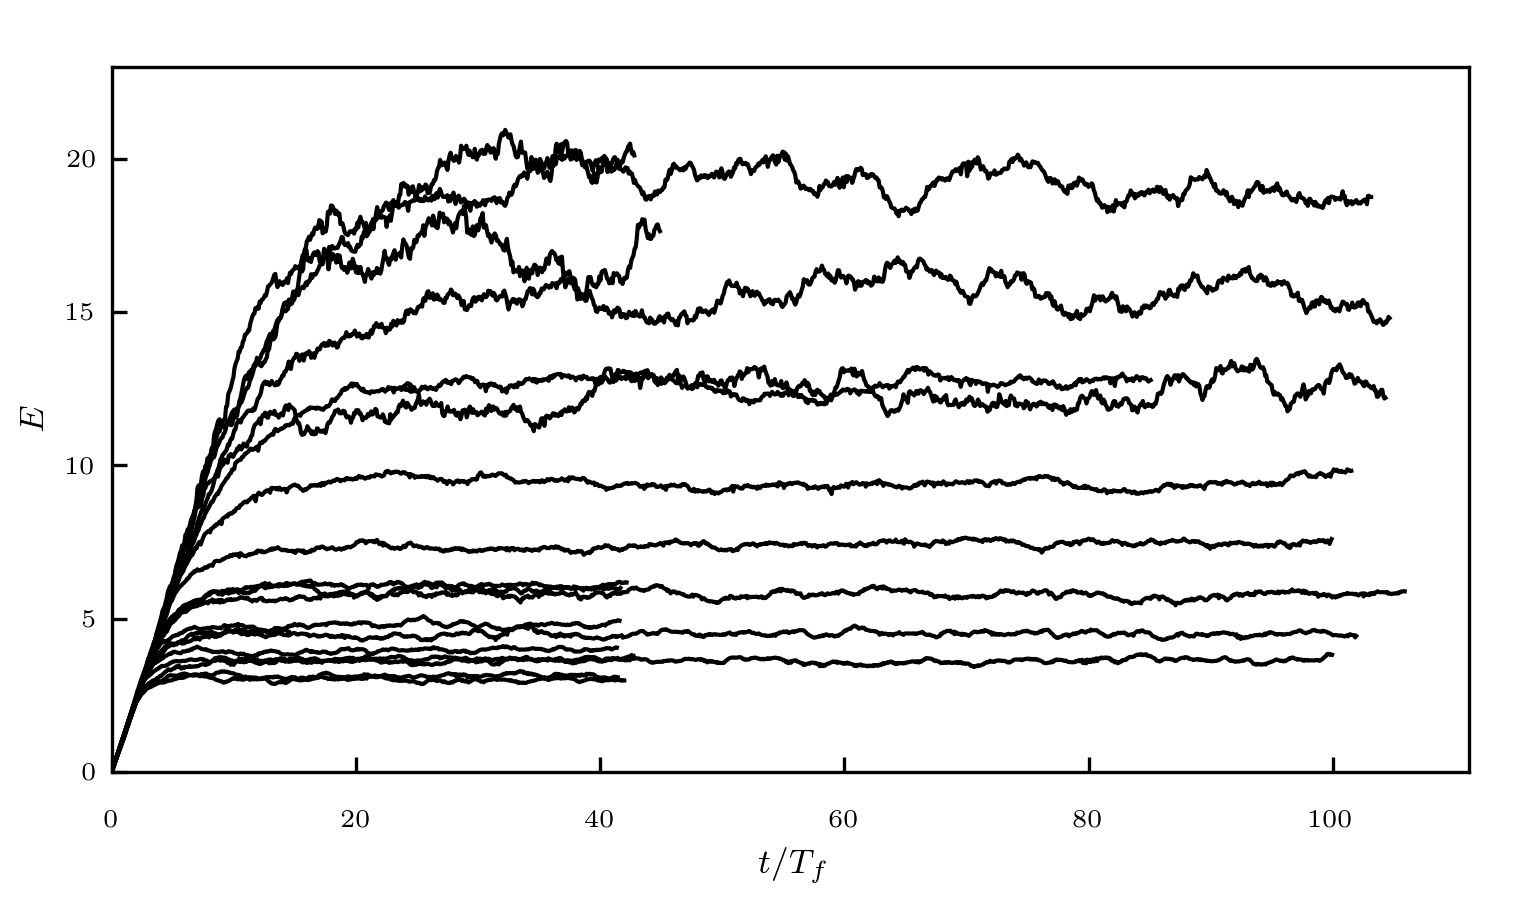
\includegraphics[width=13cm]{../Figs/fig_Emean_time}}
\centerline{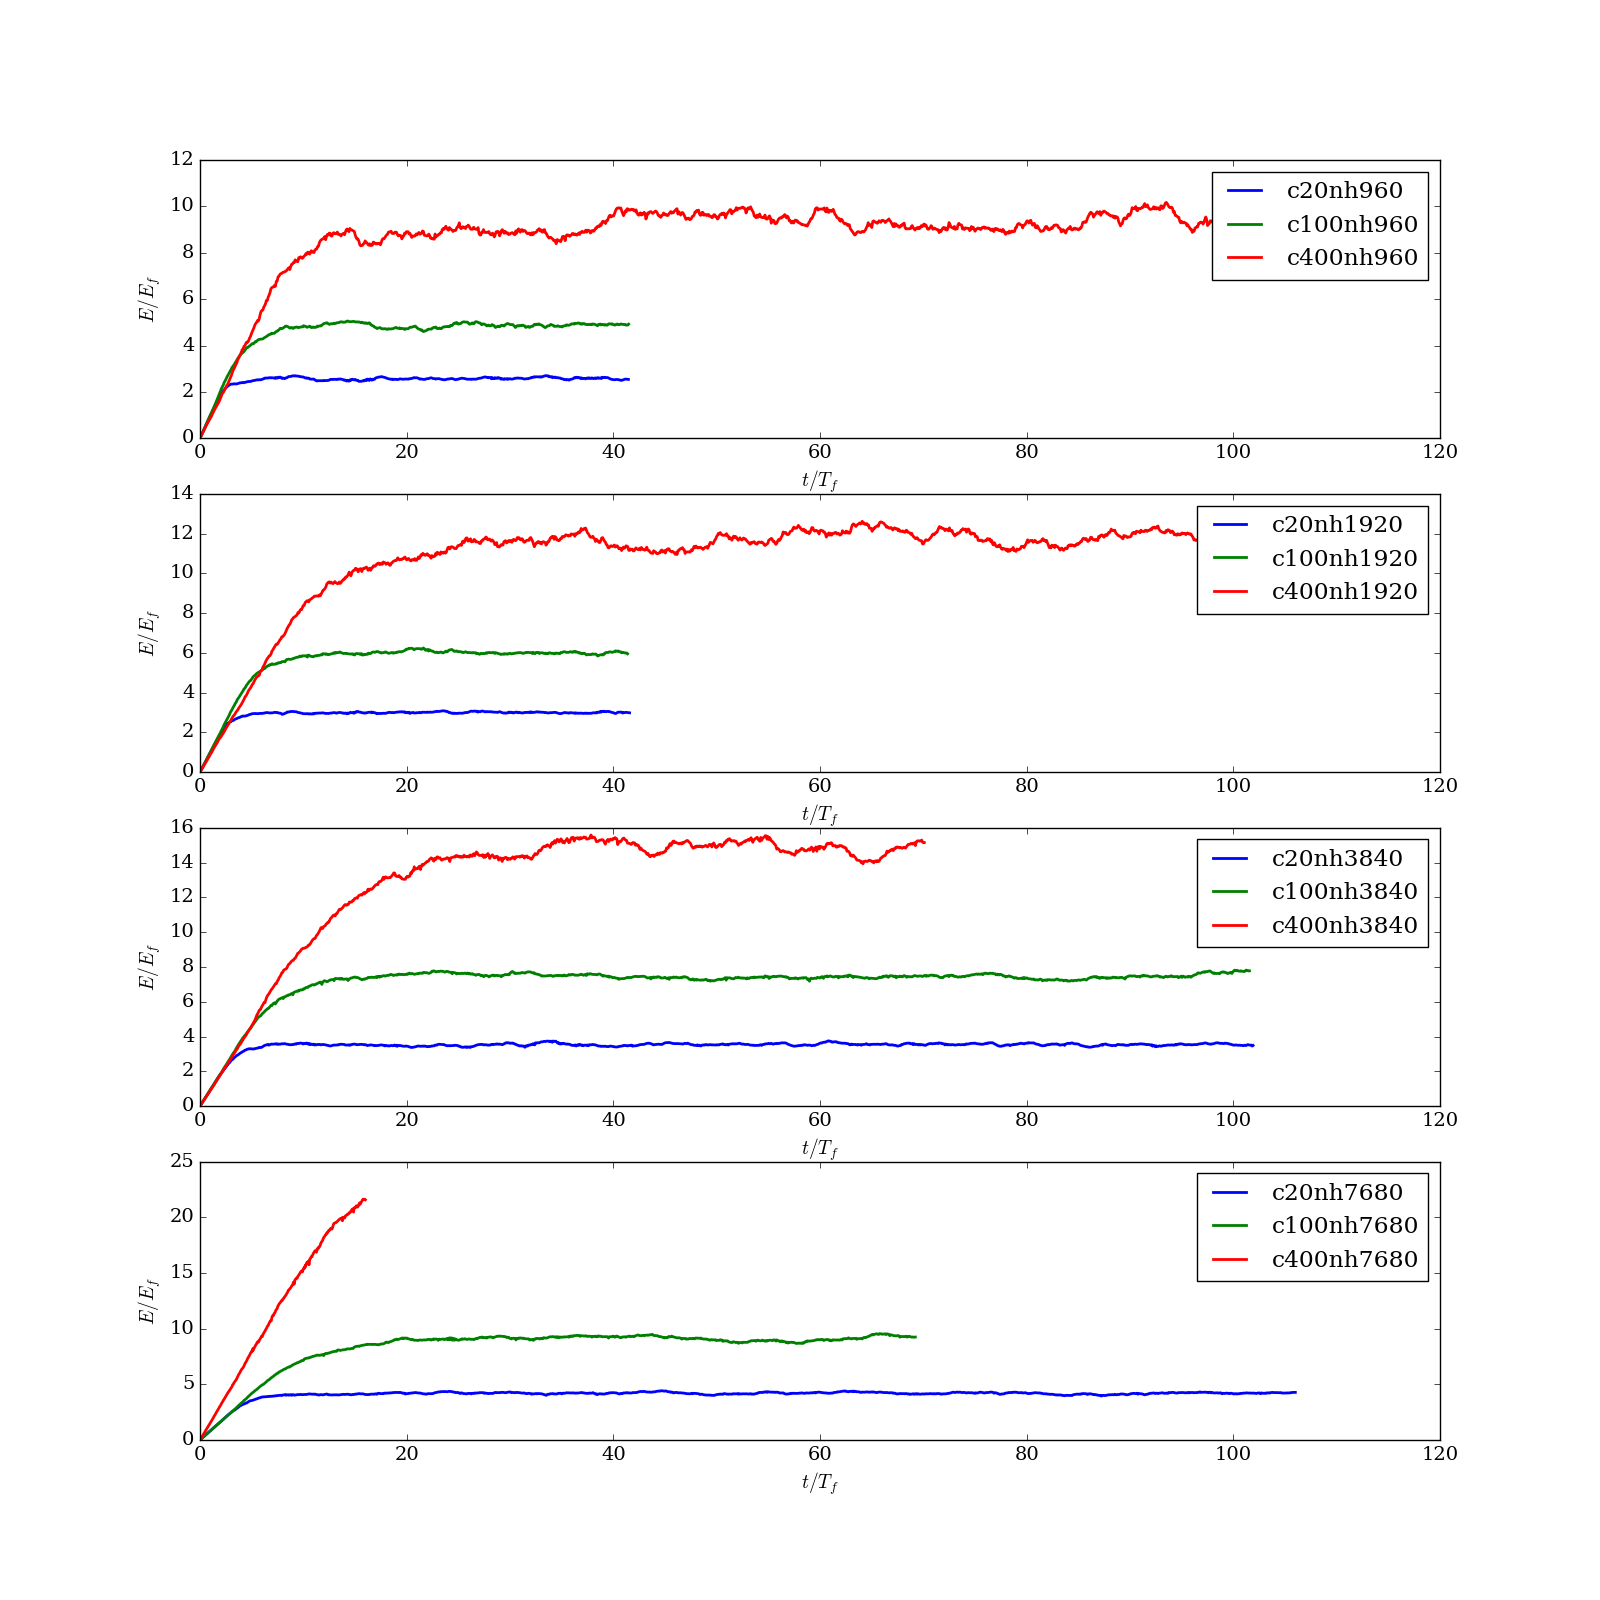
\includegraphics[width=13cm]{../Pyfig/fig_1}}
\caption{Space averaged energy 
$\langle h|\uu|^2 + c^2 h^2 \rangle/2$ versus time 
for different wave speeds $c$ and resolutions $n$.
%
The energy and the time are normalized by 
$E_f\equiv (P_0/k_f)^{2/3}$ and $T_f\equiv (P_0 {k_f}^2)^{-1/3}$,
with $P_0 = 1 \simeq \eps$.
%
The colors corresponds to different wave speeds as indicated in the figure
$c= 10$, 20, 40, 70, 100, 200, 400, 700 and 1000.
%
The different resolutions are represented by different types of lines:
\Add{thin continuous lines, $n = 240$;
thick dashed lines, $n = 480$;
thin dotted lines, $n = 960$;
thick continuous lines, $n = 1920$;
thin dashed lines, $n = 3840$;
thick dotted lines, $n = 5760$ 
and
thin dotted dashed lines, $n = 7680$.}
}
\label{fig_Evstime}
\end{figure}






The time evolution of the instantaneous total energy is shown in
figure~\ref{fig_Evstime} for different wave speeds $c$.
%
The resolution \Add{and the dissipation wave number are} progressively
increased: %
$n = 240$ ($0\leqslant t/T_f \leqslant 100$), %
$n = 480$ ($100\leqslant t/T_f \leqslant 125$), %
$n = 960$ ($125\leqslant t/T_f \leqslant 140$), %
$n = 1920$, %
$n = 3840$, %
$n = 5760$ and %
$n = 7680$\Add{, where $T_f\equiv
(P_0 {k_f}^2)^{-1/3}$ is the characteristic forcing time}.
%
Each time the resolution is increased, the energy first sharply
increases and then fluctuates.  For most of the simulations, it is
clear that a statistically stationary regime is reached.
%
However, 
%
\Remove{in the relatively short simulations at the highest
resolution for the largest wave speeds ($n = 1920$, $c = 700$ and
1000),}
%
\Add{for some relatively short simulations with very large wave speed
and/or very large resolution,}
%
there are large fluctuations and it is not absolutely certain whether
a statistically stationary regime is reached.
%
\Add{This is in particular the case for the simulations for $c = 700$, $n
= 1920$ (thick red continuous line), $c = 200$, $n = 3840$ (thin
magenta dashed line) and $c=40$, $n = 7680$ (thin blue dotted dashed
line).}
%
\Add{Note that these simulations are already quite numerically
costly. For example, the simulation for $c=1000$ and $n = 1920$
during slightly less than $20T_f$ corresponds to approximately
$8\times 10^5$ time steps.}


Since the energy is injected at large scales and dissipated only at
the smallest resolved scales, the existence of a statistically
stationary regime implies a downscale flux of energy, which is equal
to the large-scale energy injection rate.
%
For the same energy injection rate and resolution, the mean energy
increases with the wave speed, implying that when $c$ increases the
mean energy has to be larger to lead to the same downscale energy
flux.
%
The results presented in the following are from the statistically
stationary regime.  Apart from the snapshots, all shown quantities are
averaged over a period corresponding to this regime.



Table~\ref{tab} presents numerical and physical quantities for a set
of representative simulations.
%
We characterize the simulations by the forcing Froude number
\begin{equation}
F_f \Add{\equiv} \frac{\eps^{1/3}}{{k_f}^{1/3}c}.
\end{equation}
\Add{Since the characteristic forcing wave number and the dissipation
rate are approximately equal to $k_f \equiv 6 \delta k \simeq 0.75$
and $\eps \simeq P_0 = 1$, the forcing Froude number is approximately
inversely proportional to the wave speed: $F_f \simeq 1.1/c$. This
allows us to simply use the wave speed to denote the simulations.}
% where $k_f \equiv 6 \delta k = 0.75$ is a wave number characterizing
% the forcing.
%
The ratio $\kdiss/k_f$ gives an order of magnitude of the width of the
inertial range.  It is a physical quantity related to the numerical
resolution on which the flow can depend.
%
Table~\ref{tab} also displays the minimum thickness $\min(h)$
characterizing the importance of the non-quadraticity of the energy,
and $\max(|\uu|/c)$, which can be interpreted as the maximum of a
local Froude number.







%\label{section_wave_cascade_f=0}
%

\subsection{Downscale energy cascade of waves}
\label{subsection_cascade}



\begin{figure}
% \centerline{
% 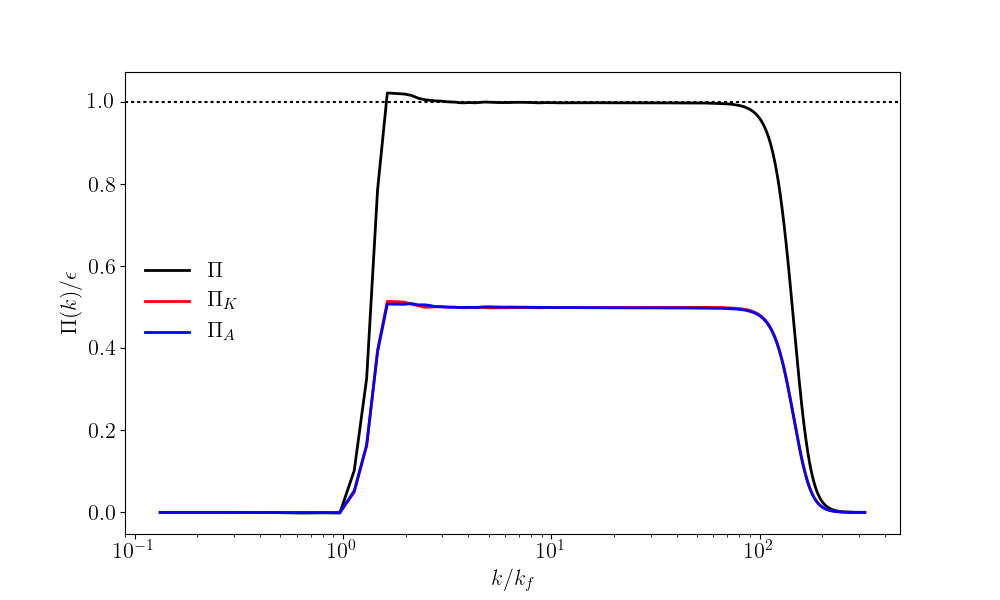
\includegraphics[width=8cm]{../Figs/fig_spect_energy_budg_c=100_N=3840}}
\caption{Spectral energy fluxes averaged over a long simulation for $c
= 100$ and $n = 3840$.  The fluxes are nondimensionalized by $\eps$
and plotted versus $k/k_f$.  }
\label{fig_seb}
\end{figure}


The spectral energy fluxes of total energy, KE and APE are plotted in
figure~\ref{fig_seb} as functions of $k/k_f$.
%
The fluxes are approximately zero at the wave numbers smaller than the
forced wave numbers.  They increase sharply at the forced wave numbers
to values close to $\eps$ for the total energy flux and to $0.5\eps$
for the KE and APE fluxes.  The fluxes then decrease to zero over the
dissipation range.
%
The energy is transferred from the forced wave numbers to the
dissipation wave numbers with a constant flux equal to the mean
forcing and dissipation rates.
%
There is an inertial range where the flux is constant and
equipartitioned between equal KE and APE fluxes.
%
However, at wave numbers $k \simeq 2 k_f$, the flux is not exactly
equal to $\eps$.  This is very likely related to the energy injection
at wave numbers for which the force is zero, which is due to the
non-quadraticity of the kinetic energy (see appendix~\ref{app_comp}).
%
Nevertheless this effect is non-negligible only for wave number of the
order of $k\simeq 2 k_f$, i.e.\ at the first harmonics of the forced
wave numbers, such that there is a clear and wide inertial range
between $k\gtrsim 3 k_f$ to the dissipation range starting at wave
number of the order of $k \sim 70 k_f$.




\begin{figure}
% \centerline{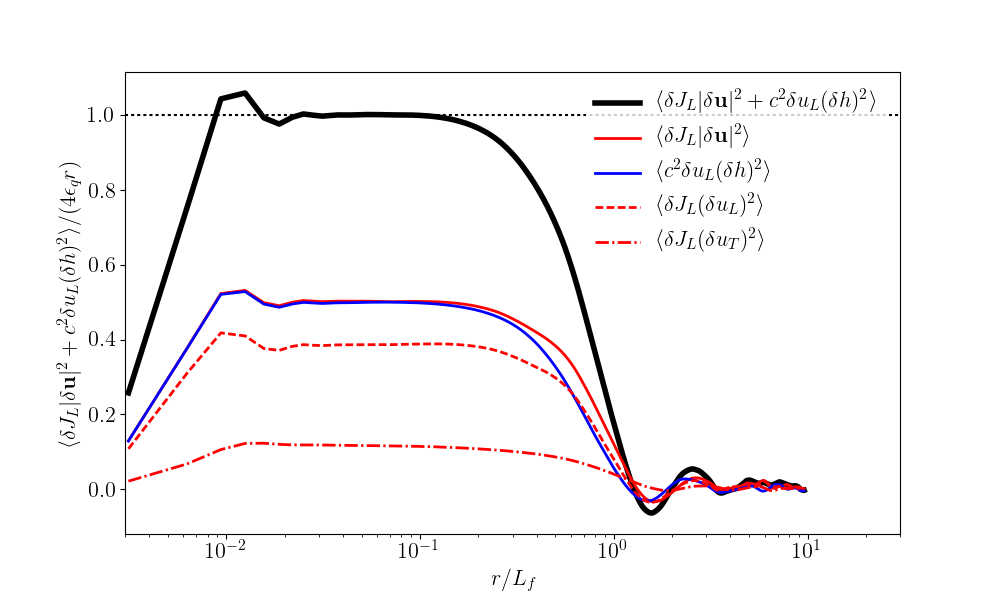
\includegraphics[width=8cm]{../Figs/fig_Kolmo_c=20_N=3840}}
\caption{
Third order structure functions involved in the exact Kolmogorov law (\ref{eq_Kolmo}) 
averaged over a long simulation for $c = 20$ and $n = 3840$.
%
The structure functions are normalized by $4 \eps r$.
%
Black thick line, $\mean{ \delta J_L|\delta \uu|^2 } 
+ c^2\mean{\delta u_L(\delta h)^2}$;
light thin line, $c^2\mean{\delta u_L (\delta h)^2}$;
dark thin line, $\mean{\delta J_L |\delta \uu|^2}$.
%
The dotted straight line shows $4 \eps_q r$, 
where $\eps_q$ is the quadratic energy dissipation rate.
}
\label{fig_Kolmo}
\end{figure}


Figure~\ref{fig_Kolmo} shows the quantity $\mean{\delta J_L|\delta
\uu|^2 } + c^2\mean{\delta u_L(\delta h)^2 }$ (black thick line)
normalized by $4 \eps r$ for $c = 20$ and $n = 1920$.
%
In this section, the brackets $\mean{}$ denote the average over space
and time.
%
The dotted straight line shows the quantity $4 \eps_q r$, where
$\eps_q$ is the quadratic energy dissipation rate (see
appendix~\ref{app_comp}) which takes place at small scales.
%
We see that the Kolmogorov law (\ref{eq_Kolmo}) is well satisfied
between \Add{$r \simeq 0.02L_f$ and $r \simeq 0.1 L_f$}.  The dark and
light thin continuous lines correspond to the quantities $\mean{\delta
J_L|\delta \uu|^2 }$ and $c^2\mean{\delta u_L(\delta h)^2}$,
respectively.
%
These two quantities are nearly equal over the inertial and
dissipation ranges, which is consistent with a wave cascade when
$f=0$.
%
The agreement with the Kolmogorov law and the equality between
$\mean{\delta J_L|\delta \uu|^2 }$ and $c^2\mean{\delta u_L(\delta
h)^2}$ are the equivalents in the separation space of the plateau in
the total energy flux and the equality between $\Pi_K$ and $\Pi_A$,
respectively.




\begin{figure}
% \centerline{
% \includegraphics[width=8cm]{../Figs/fig_spatiotempspectra_c=20_Nh=3840}}
\caption{Spatio-temporal spectra of KE (dark lines) and APE (light
lines) for $c = 20$ and $n = 3840$ versus $\omega/\omega_l$, where
$\omega_l = c k$.  From the larger to the smaller spectra, $k/\delta k
= 12$, 27, 62, 143, 327, and 746.  }
\label{fig_spatiotemp_spectra}
\end{figure}

Figure~\ref{fig_spatiotemp_spectra} presents the spatio-temporal
spectra plotted as a function of the normalized frequency
$\omega/\omega_l$.
%\PA{Explain how these spectra have been calculated.}  
In order to calculate these spectra, we have saved well-resolved time
series of $\hat d(\kk)$ and $\hat a(\kk)$ for wave numbers inside
particular shells such as $k\leqslant \kk<k+\delta k$, computed the
temporal spectrum of each signal and averaged over the wave numbers
inside each shell.
%
The spectra are strongly dominated by large peaks at $\omega =
\omega_l$ indicating that the characteristic frequency for each wave
number is the linear frequency.  However, the widening of the peaks
can be explained only by nonlinear effects.  \Add{The equipartition
between kinetic and potential energies is expected since the flow only
consists of gravity waves and the total energy is nearly equal to the
quadratic energy which is equal to the sum over all waves of their
equipartitioned quadratic energy.}












\subsection{Time- and space-averaged energy as a function of $c$}

\begin{figure}
% \centerline{
% \includegraphics[width=\halfwidth]{../Figs/fig_Emean_c}
% \includegraphics[width=\halfwidth]{../Figs/fig_Emean_resol}
% }
\caption{Time- and space-averaged energy 
$\langle h|\uu|^2 + c^2 h^2 \rangle/2$ 
of the statistically stationary flows.
%
In (\textit{a}), the energy is divided by 
$\sqrt{\eps}$ and plotted versus $c$ for 3 resolutions:
$n = 960$, dotted lines; 
$n = 1920$, continuous lines and 
$n = 3840$, dashed lines. 
The cyan curves show the law $C_n \sqrt{\eps L_f c}$, 
with $C_n$ a fit coefficient.
%
In (\textit{b}), the energy is divided by 
$\sqrt{\eps L_f c}$ and plotted versus $n$
for six values of $c$ as indicated in the legend.
}
\label{fig_Evsc}
\end{figure}


Figure~\ref{fig_Evsc}(\textit{a}) shows the time- and space-averaged
energy for the statistically stationary flows divided by the square
root of the mean energy dissipation rate as a function of $c$ and for
three resolutions: $n = 960$, dotted lines; $n = 1920$, continuous
lines and $n = 3840$, dashed lines.
%
For all resolutions, the energy increases with $c$.  More precisely,
the curves can be well fitted to a law $E = C_n \sqrt{\eps L_f c}$
(blue lines).  However, the coefficient $C_n$ varies with the
resolution, i.e.\ with the effective Reynolds number.
%
This is very different from the case of isotropic turbulence where the
energy scales as $E \sim (\eps L_f)^{2/3}$ and does not vary with the
Reynolds number in the limit of very large Reynolds number.
%
Weak wave turbulence theory predicts an energy-flux law of the form $E
\propto \eps^{1/(N-1)}$, where $N$ is the number of waves involved
in the nonlinear interactions \cite[]{Nazarenko2011}.  Therefore, the
scaling $E = C_n \sqrt{\eps L_f c}$ would correspond to interactions
involving three waves.
%
However, the hypothesis needed for applying the weak wave turbulence
formulation are not fulfilled.


This effect of the increase of the energy with the resolution is
investigated in figure~\ref{fig_Evsc}(\textit{b}) where the quantity
$C_n = E/\sqrt{\eps L_f c}$ is plotted as a function of the
resolution.
%
For $c = 10$ (dotted line), the waves are not very fast and the
variation with the resolution is weak.
%
However, in the limit of very fast waves ($c>100$), the curves for the
different wave speeds nearly collapse and increase at least up to $n =
5760$.  The increase tends to saturate but it is difficult to know
from our results what is the scaling of $C_n$ as a function of the
resolution and if it really saturates for very large $n$ and $c$.
%
In order to decide on this issue, we would need to run simulations in
the very-fast-wave regime, $c>100$, and at very large resolutions $n >
5760$.  In this regime the energy fluctuations are large so
that the simulations would have to be carried out for very long time
in order to get a good convergence for the mean energy.  Since the
time step has to be extremely small in this regime, such simulations
would be too costly.





\subsection{Energy spectra}


We now turn to the study of the energy spectra.  A dimensional
analysis based on the assumption that the spectra only depend on
$\eps$, $c$ and $k_f$ gives the following general expression
\begin{equation}
E_{\alpha, \beta}(k) = k^{-\alpha} \eps^\beta   c^{2- 3\beta} 
{k_f}^{\alpha -1 - \beta}, \label{eq_E_alpha_beta}
\end{equation}
where $\alpha$ and $\beta$ are two free parameters.



\begin{figure}
% \centerline{
% \includegraphics[width=\halfwidth]{../Figs/fig_spectra_c_Nx=1920_k32}
% \includegraphics[width=\halfwidth]{../Figs/fig_spectra_c_Nx=3840_k32}
% }
% \centerline{
% \includegraphics[width=\halfwidth]{../Figs/fig_spectra_c_Nx=1920_k2}
% \includegraphics[width=\halfwidth]{../Figs/fig_spectra_c_Nx=3840_k2}
% }
\caption{
Compensated energy spectra versus $k/k_f$ for different wave speeds $c$.
%
The spectra are compensated by $k^{-3/2}\sqrt{\varepsilon c} $ 
in (\textit{a,b})
and by $k^{-2}c^{1/3} \eps^{5/9} k_f^{4/9} $ 
in (\textit{c,d}).
%
The resolution is 
$n = 1920$ in (\textit{a,c}) and 
$n = 3840$ in (\textit{b,d}).
%
In (\textit{a,c}), the wave speed goes from 10 to 1000
and 
in (\textit{b,d}) from 10 to 200 
(for the precise values, see figure~\ref{fig_Evstime}).
}
\label{fig_spectra_c}
\end{figure}


The scaling of the energy as $\sqrt{\eps L_f c}$ suggests that the
spectra should scale like the Zakharov-Sagdeev spectrum, $E(k) \sim
k^{-3/2}\sqrt{\eps c}$, which is the prediction of weak wave
turbulence theory for three-dimensional acoustic turbulence
\cite[]{Nazarenko2011}.
%
The compensated spectra $E(k) / ( k^{-3/2}\sqrt{\eps c})$ are plotted
in figure~\ref{fig_spectra_c}(\textit{a}) for $n = 1920$ and in
figure~\ref{fig_spectra_c}(\textit{b}) for $n = 3840$.  The different
curves correspond to different wave speeds, going from $c=10$ to
$c=1000$ for $n = 1920$ and from $c=10$ to $c=200$ for $n = 3840$.
%
For both resolutions, the compensated spectra collapse at the
energy-dominating small wave numbers.
%
However, these compensated spectra are not flat in the inertial range
and do not collapse in the inertial and dissipation ranges, i.e. for
$k\gtrsim 2k_f$.  In the inertial range, they follow a clear $k^{-2}$
scaling law and there is a bottleneck in the dissipation range where
the slope is close to $-3/2$.
%
\cite{Kuznetsov2004} showed that $k^{-2}$ spectra can be explained by
singularities and this scaling has already been observed in
two-dimensional acoustic turbulence \cite[]{FalkovichMeyer1996}.
%

Inserting $\alpha = 2$ in the spectrum (\ref{eq_E_alpha_beta}) gives
\begin{equation}
E_\beta(k) = k^{-2} {k_f}^{1-\beta} c^{2-3\beta} \eps^\beta  
\end{equation}
and we have found that the numerical spectra are very close to the
spectrum $E_\beta(k)$ with $\beta = 5/9$.
%
The compensated spectra $E(k) / ( k^{-2} c^{1/3} \eps^{5/9} k_f^{4/9}
)$ are plotted in figure~\ref{fig_spectra_c}(\textit{c}) for $n =
1920$ and in figure~\ref{fig_spectra_c}(\textit{d}) for $n = 3840$.
The collapse is very good in the inertial range but we stress that we
are not aware of any theory predicting the empirical spectrum $k^{-2}
c^{1/3} \eps^{5/9} k_f^{4/9}$.





\begin{figure}
% \centerline{\includegraphics[width=8cm]{../Figs/fig_spectra_c=40_nh=7680}}
\caption{Compensated spectra
of total energy (thick black line)
kinetic energy (thin dark line) and
available potential energy (thin light line)
for $c = 40$ and $n = 7680$.}
\label{fig_spectra_c40}
\end{figure}

Figure~\ref{fig_spectra_c40} shows the compensated spectra $E(k) / (
k^{-2} c^{1/3} \eps^{5/9} k_f^{4/9} )$ of total energy (black line),
KE (red line) and APE (blue line) for $c = 40$ and $n = 7680$.  For
all wave numbers, we have $E(k) = 2E_K(k) = 2E_A(k)$ since the flow
only consists of \Add{gravity} waves.
%
The spectra are very close to $k^{-2}$ in the inertial range over more
than one decade and the shallowing to a slope close to $-3/2$ is
clearly confined to the dissipation range.  This confirms that this
bump is due to a dissipation effect and that there is no wide
$k^{-3/2}$ spectrum even at very large resolutions.


% \begin{figure}
% \centerline{
% \includegraphics[width=\halfwidth]{../Figs/fig_spectra_resol_c=10}
% \includegraphics[width=\halfwidth]{../Figs/fig_spectra_resol_c=40}
% }
% \caption{Compensated energy spectra $E(k) / ( k^{-3/2}\sqrt{\eps c})$
% for different resolutions.  In (\textit{a}), $c = 10$ and in
% (\textit{a}), $c = 40$.}
% \label{fig_spectra_resol}
% \end{figure}

% The compensated spectra $E(k) / ( k^{-3/2}\sqrt{\eps c})$ are plotted
% for different resolutions %
% in figure~\ref{fig_spectra_resol}(\textit{a}) for $c=10$ and 
% in figure~\ref{fig_spectra_resol}(\textit{b}) for $c=40$.
% %
% We see that an inertial range with a $k^{-2}$ scaling starts to appear
% for $n\gtrsim 960$.
% %
% As seen in figure~\ref{fig_Evsc}, the ratio $E/\sqrt{\eps L_f c}$ only
% weakly varies for $c=10$ but increases in the fast-waves regime for
% $c=40$.  This effect can be seen here at the energy-containing wave
% numbers $k<2 k_f$.  However, the variation with the resolution is much
% weaker in the inertial range at $k>2 k_f$.



In subsection~\ref{subsection_cascade}, we have shown that third-order
structure functions scale like $r$ since there is a downscale energy
cascade.
%
The Kolmogorov method predicts $k^{-5/3}$-spectra but the numerical
spectra are much steeper in the inertial range, with a slope equal to
-2.  The fact that third-order and second-order quantities can not be
simply related by the Kolmogorov scaling implies that the cascade is
very intermittent.




\subsection{Effect of the shocks and intermittency}




\begin{figure}
\setlength{\halfwidth}{69mm}
% \centerline{
% \includegraphics[width=\halfwidth]{../Figs/fig_2Dh_c20}
% \hspace{-4mm}
% \includegraphics[width=\halfwidth]{../Figs/fig_2Dh_c200}
% }
% \centerline{
% \includegraphics[width=\halfwidth]{../Figs/fig_2Duy_c20}
% \hspace{-4mm}
% \includegraphics[width=\halfwidth]{../Figs/fig_2Duy_c200}
% }
\caption{
Snapshots for $n = 1920$ and two values of the wave speed 
$c= 20$ (\textit{a,c}) and $c= 200$ (\textit{b,d}).
The colors represent the thickness in (\textit{a,b}) and
the $y$-component of the velocity in (\textit{c,d}).
The arrows represent the velocity field.
%
The coordinates are nondimensionalized by the characteristic scale of
the forcing $L_f = 3.57$.  }
\label{fig_phys}
\end{figure}

Figure~\ref{fig_phys} shows %
the normalized thickness $h$ %
(figures~\ref{fig_phys}\textit{a,b}) %
and the $y$-component of the velocity $u_y$ %
(figures~\ref{fig_phys}\textit{c,d}) %
for $c = 20$ (figures~\ref{fig_phys}\textit{a,c}) and %
$c = 200$ (figures~\ref{fig_phys}\textit{b,d}).
%
These wave speeds correspond %
to a moderate forcing Froude number $F_f \sim 0.05$ and %
to a very small forcing Froude number $F_f \sim 0.005$, respectively.
The normalized surface displacement $\eta = h - 1$ is of order 0.3 for
$c = 20$ and one order of magnitude smaller, 0.03, for $c = 200$.
%
The typical velocity is also much smaller than the wave speed, %
with $u_y/c \sim 0.2$ for $c = 20$ %
and $u_y/c \sim 0.03$ for $c = 200$. %
This confirms that the flows are in a fast-wave regime, especially for
$c = 200$.
%
However, many discontinuities can be seen in both fields $h$ and
$u_y$.  These discontinuities are hydraulic jumps, which are the
equivalent to shocks in a compressible flows.
%
\Add{Baines (1998) provides a theoretical prediction for the velocity
of the hydraulic jumps is one-layer shallow-water flow:
\begin{equation}
c_s = c \sqrt{\frac{h_+}{h_-} \frac{h_+ + h_-}{2}},
\end{equation}
where $h_+$ and $h_-$ are the dimensionless thickness before and after
the jump.
%
We have verified that the velocity of the discontinuities in the
simulations is consistent with this theoretical prediction, implying
that the associated Froude number (or Mach number) is of the order
unity.}

\nocite{Baines1998}

% We have verified that these shocks are very fast and travel at a
% velocity of the order of the wave speed \Add{(more precisely, Baines 1998)}
% , implying
% that their associated Froude number (or Mach number) is of the order
% unity.
%el (This is not necessarily true...)
% The existence of shocks implies that there is a strong coherence
% between small and large wave numbers and indicates nonlocal
% interactions between wave numbers.
%
In between the shocks, the flow is very smooth for $c=20$ and slightly
more irregular for $c = 200$.

Figures~\ref{fig_phys}(\textit{c,d}) display the $y$-component of the
velocity.  There are less discontinuities in this quantity than in the
thickness. More precisely, the $h$-discontinuity lines that are along
the $y$-axis are not associated with corresponding discontinuities of
the $y$-component of the velocity. This can be seen for example for
the shock at $x/L_f\simeq 0.4$ and $y/L_f\simeq 2.1$ in
figures~\ref{fig_phys}(\textit{a}) and \ref{fig_phys}(\textit{c}).
%
This illustrates that the singularity in the velocity is in the
component perpendicular to the shock line, which is the assumption on
the structure of the velocity discontinuities used in the model
presented in \S~\ref{subsection_shock_model}.







\begin{figure}
% \centerline{
% \includegraphics[width=\halfwidth]{../Figs/fig_interm_strfct_ux}
% \includegraphics[width=\halfwidth]{../Figs/fig_interm_strfct_uy}
% }
\caption{
Compensated fifth-order structure functions $\mean{|\delta u_L|^5}/r$ 
of (\textit{a}) the longitudinal increments and (\textit{b}) the
transverse increments. %
The crosses indicate the range of separation $r$ where the exponent
$\zeta_p$ is computed. %
The dashed lines correspond to the Kolmogorov scaling laws $r^{p/3}$
and $\zeta_p = p/3$.  The wave speed and the resolution are $c = 40$
and $n = 7680$.  }
\label{fig_strfct5}
\end{figure}


The shock model derived in subsection~\ref{subsection_shock_model}
predicts that structure functions of all orders should scale linearly
with $r$.
%
Figure~\ref{fig_strfct5} presents fifth-order structure functions
compensated by $r$.
%
Figures~\ref{fig_strfct5}(\textit{a}) and
\ref{fig_strfct5}(\textit{b}) correspond to the structure functions
computed from the longitudinal increments and the transverse
increments, respectively.  The structure functions compensated by $r$
are nearly flat between $r \simeq 0.012 L_f$ and $r \simeq 0.06 L_f$,
showing that they scale like $r$ on this relatively narrow range of
scale compared to the inertial range.
%
The $r$-scaling is very different from the slope of the fifth-order
structure functions calculated from the Kolmogorov scaling $\zeta_5 =
p/3 \simeq 1.66$ (dashed straight line).  This shows that the wave
cascade is strongly intermittent and that this intermittency can be
explained by the presence of discontinuities related to the shocks.




\begin{figure}
% \centerline{
% \includegraphics[width=\halfwidth]{../Figs/fig_interm_ux}
% \includegraphics[width=\halfwidth]{../Figs/fig_interm_uy}
% }
\caption{
Exponents $\zeta_p$ of the structure functions 
of (\textit{a}) the longitudinal increments 
and (\textit{b}) the transverse increments versus the order $p$.
%
The dashed lines correspond to 
the Kolmogorov scaling laws $r^{p/3}$ and $\zeta_p = p/3$.
The wave speed and the resolution are $c = 40$ and $n = 7680$.
}
\label{fig_interm}
\end{figure}






The slope of the structure functions of order $p$ over the range
$0.012 L_f\leqslant r \leqslant 0.06 L_f$, $\zeta_p$, are plotted in
figure~\ref{fig_interm}(\textit{a}) for the longitudinal increments
and in figure~\ref{fig_interm}(\textit{b}) for the transverse
increments.
%
The exponent are very far from the Kolmogorov scaling $\zeta_p = p/3$.
They increase as $p$ for $p\ll1$, saturate to a value close to 1 for
$p>2$ and tend to decrease for $p>3$.
%
A similar shape of the $\zeta_p$ function has been predicted for
Burger turbulence \cite[]{BouchaudMezardParisi1995}.
%
The shape of $\zeta_p$ at very small $p$ is determined by the
scaling of the smallest velocity increments and the $p^1$-variation
shows that these smallest increments scales like $\delta u \sim r^p$.
%
The plateau at $p > 2$ is a consequence of the dominance by shocks of
the largest increments.
%
Note that these results are obtained for a relatively small forcing
Froude number $F_f \simeq 0.03$ corresponding to $c=40$.  The function
$\zeta_p$ has approximately the same extreme shape for a larger Froude
number $F_f \simeq 0.01$, corresponding to $c=10$.  Note also that the
decrease of $\zeta_p$ for $p>3$ is anomalous, which could be due to
the relatively narrow width of the range over which $\zeta_p$ is
computed.



\begin{figure}
% \centerline{
% 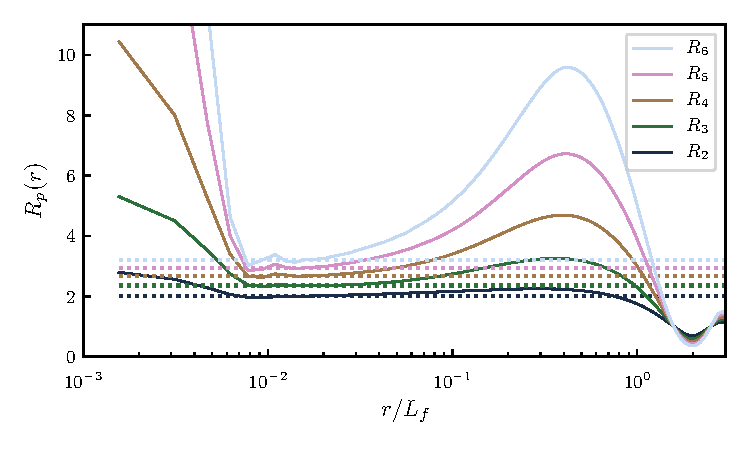
\includegraphics[width=\halfwidth]{../Figs/fig_ratio_strfct}
% }
\caption{
Ratio of the structure functions of the velocity increments 
$R_p(r) \equiv \mean{|\delta u_L|^p} / \mean{|\delta u_T|^p}$
for $p = 2,$ 3 and 4.
The dotted straight lines indicate the values computed by the shock model:
$R_2 = 2$, $R_3 = 6\pi/8$ and $R_4 = 8/3$.
%
The wave speed and the resolution are $c = 10$ and $n = 7680$.  }
\label{fig_ratio}
\end{figure}


The functions $R_p = \mean{|\delta u_L|^p}/\mean{|\delta u_T|^p}$ are
plotted in figure~\ref{fig_ratio} for $p =2$ to 4.  The predictions of
the shock model, $R_2 = 2$, $R_3 = 6\pi/8$ and $R_4 = 8/3$, are also
plotted in dotted lines for comparison.  We see that the numerical
results are reasonably close to these predictions.  However, the
agreement is less good for smaller Froude number (not shown).  The
structure functions are fully determined by shocks only for Froude
numbers that are not too small, which is consistent with the snapshots
in figure~\ref{fig_phys} showing that the fields between the shocks
are more irregular for the smallest Froude number.


\begin{figure}
% \centerline{
% 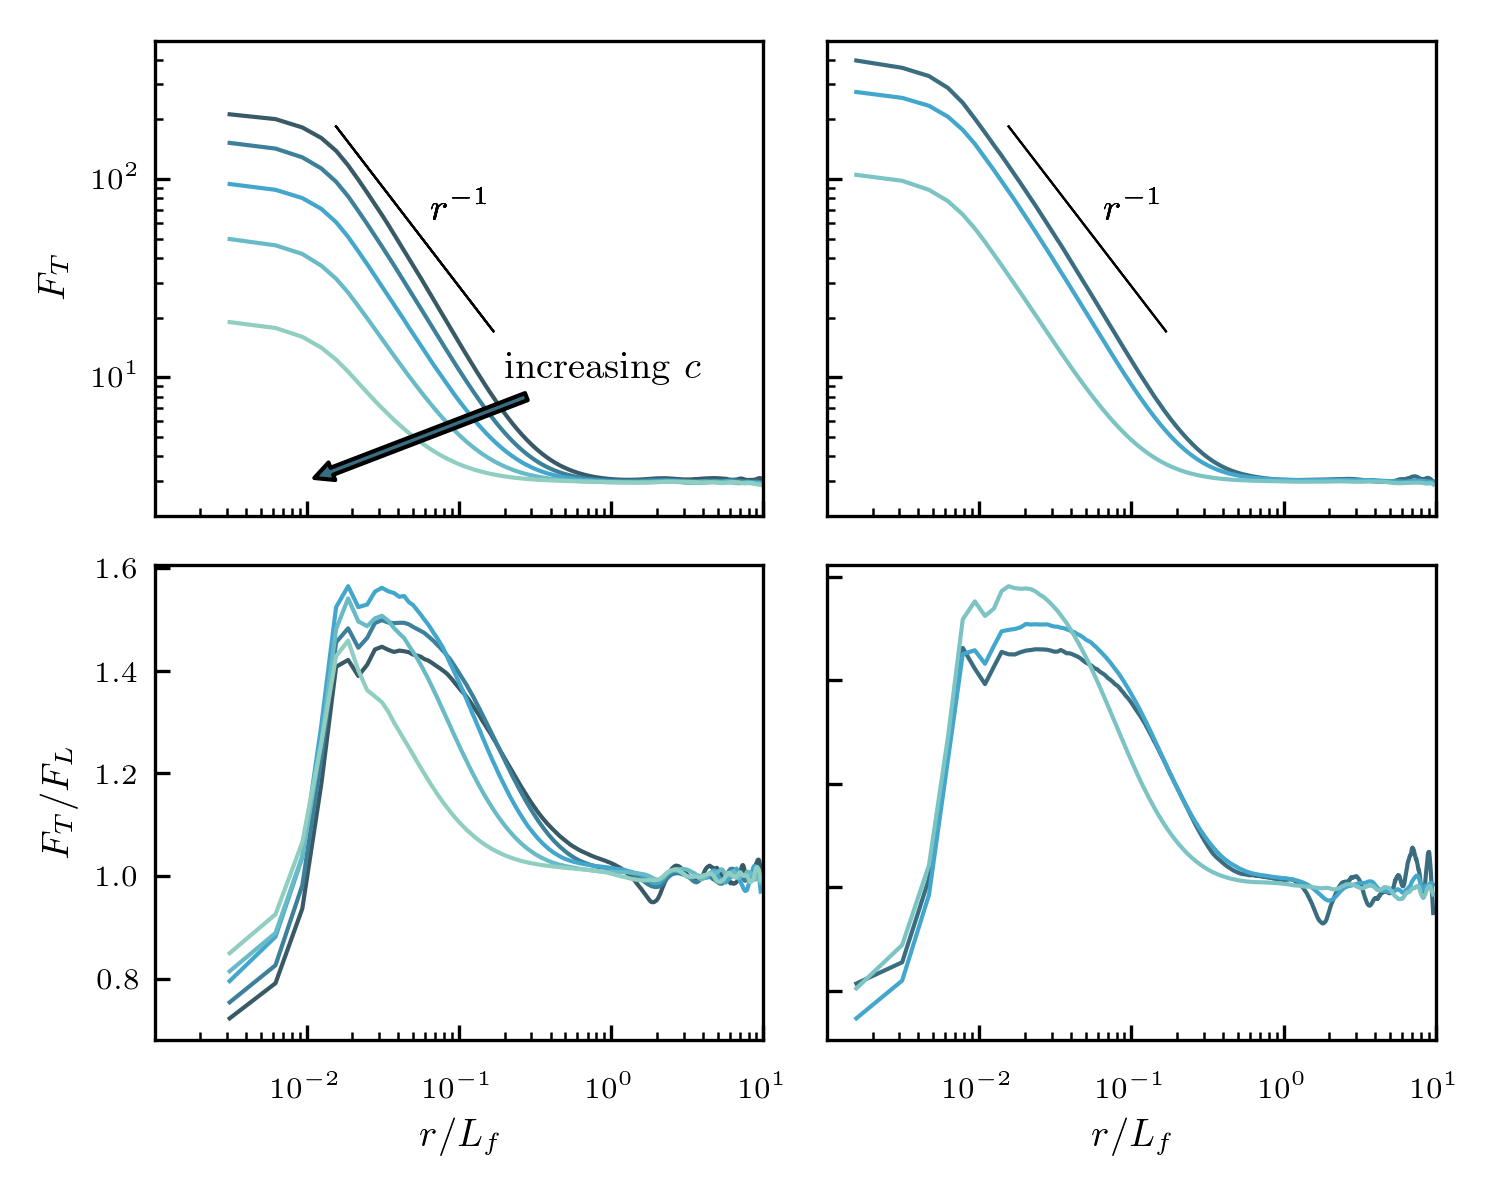
\includegraphics[width=\halfwidth]{../Figs/fig_flatness}
% }
\caption{ Flatness of the longitudinal and transverse increments for
$c = 10$ and $n = 7680$. The straight continuous lines indicate the
$r^{-1}$-scaling and the straight dashed line the $r^{-3/2}$-scaling.
The inset shows the ratio $F_T/F_L$ and the corresponding value
computed by the shock model, $F_T/F_L = 1.5$.  }
\label{fig_flatness}
\end{figure}
%
Figure~\ref{fig_flatness} shows the flatness of the longitudinal and
transverse increments, computed from a numerical simulation for $c =
10$ and $n = 7680$.
%
For a Gaussian probability distribution the flatness factor is equal
to 3 whereas the shock model predict flatness factors scaling like
$r^{-1}$.
%
We see that here the flatness factors are much larger than 3, of the
order of $10^3$.
%
Remarkably, they scale approximately as $r^{-1}$ as predicted by the
shock model and the ratio $F_T/F_L$ is very close to the predicted
value 1.5.



% Figure~\ref{fig_flatness}(\textit{b}) shows the same quantities
% computed from atmospheric data measured by commercial aircraft.
% %
% The flatness curves have been taken from \cite{Lindborg1999}.
% Surprisingly, the atmospheric results are quite similar to the
% numerical ones. The flatness factors are very large and strongly
% decrease at scales smaller than 100 km.  Interestingly, the ratio
% $F_T/F_L$ is also very close to the value 1.5 predicted by the shock
% model.
% %
% We stress that even though these similarities are striking, the
% underlying dynamics are very different.
% %
% While there is no energy in the quasi-geostrophic modes in the
% numerical simulations, the atmospheric flows are usually close to be
% quasi-geostrophic at horizontal scales larger than 500 km and the
% vertical vorticity is in average of the same order of magnitude than
% the horizontal divergence at the mesoscales, i.e. at horizontal scales
% between 10 and 500 km \cite[]{Lindborg2007jas}.
% %
% Therefore, it is not surprising to also see differences between the
% atmospheric and the numerical results. The flatness factors in
% figure~\ref{fig_flatness}(\textit{b}) vary approximately as $r^{-3/2}$
% (dashed line), which is significantly faster than for the numerical
% simulations of the shallow-water model. Moreover, the second-order
% structure functions in the atmosphere scale as $r^{2/3}$
% \cite[]{Lindborg1999, ChoLindborg2001,
% FrehlichSharman2010}. Considering the scaling for the flatness
% factors, this implies that the variation with scale of the
% fourth-order structure functions is actually very weak, which is
% not in agreement with the prediction of the shock model.
% %
% Nevertheless, we do not know other explanations of such very large
% flatness factors with a ratio $F_T/F_L=1.5$ observed in the atmosphere.
% %
% Thus, we think that these results raise interesting questions
% regarding the interpretation of structure functions measured in the
% atmosphere.  How important are the discontinuities on horizontal
% cross-sections in these cases?
% %
% It is well known that the fronts separating cold and warm regions 
% explain many meteorological phenomena.
% %
% The curves in figure~\ref{fig_flatness} seem to indicate that 
% they could also have strong effects on the statistics of the atmosphere
% over a quite large range of scales.











%\section{Effects of global rotation}
%\label{section_rotation}
%


In order to study the effects of system rotation, we have carried
out four supplementary simulations for $c = 20$, $n = 1920$ and
constant and non-zero Coriolis parameter $f$.  The values of $f$ have
been chosen such that to yield relatively small Rossby numbers
\begin{equation}
Ro_f = \frac{\eps^{1/3} {k_f}^{2/3}}{f} \lesssim 0.1,
\end{equation}
and to span a range of Burger number,
\begin{equation}
Bu = \left(\frac{k_f}{k_d}\right)^2 = \left(\frac{Ro_f}{F_f}\right)^2,
\end{equation}
going from 0.5 to 4.  For these moderate values of global rotation, a
statistically stationary regime is also reached.  Table~\ref{tab_rot}
displays the parameters for these simulations.
\begin{table}
\begin{center}
\begin{tabular}{cc@{\hskip 8mm}c@{\hskip 8mm}ccc@{\hskip 8mm}cccc@{\hskip 8mm}cc}
$n$ & $c$ & $\nu_8$ & $f$ & $Ro$ & $Bu$ & $\eps$ & $\displaystyle\frac{\kmax}{\kdiss}$ & $\displaystyle\frac{\kdiss}{k_f}$ & $F_f$ & $\min h$ & $\displaystyle\frac{\max |\uu|}{c}$ \\[3mm]
1920 &   20 & 9.6e-13 &  0   &  $\infty$ & $\infty$ & 0.99 & 2.46 &  58 &  0.055 & 0.59 & 0.56 \\
1920 &   20 & 9.6e-13 &  7.5 &   0.11 &      4 & 0.96 & 2.47 &  58 &  0.054 & 0.67 & 0.52 \\
1920 &   20 & 9.6e-13 & 10.7 &  0.076 &      2 & 0.93 & 2.47 &  58 &  0.054 & 0.70 & 0.62 \\
1920 &   20 & 9.6e-13 & 15.1 &  0.052 &      1 & 0.85 & 2.48 &  57 &  0.052 & 0.70 & 0.65 \\
1920 &   20 & 9.6e-13 & 21.3 &  0.037 &    0.5 & 0.84 & 2.48 &  57 &  0.052 & 0.66 & 0.81 \\
\end{tabular}
\caption{Overview of parameters for the simulations used to study the effect of rotation. 
}
\label{tab_rot}
\end{center}
\end{table}



\begin{figure}
\centerline{
\includegraphics[width=\halfwidth]{../Figs/fig_Emean_f}
\includegraphics[width=\halfwidth]{../Figs/fig_spectra_f_Nx=1920}
}
\caption{Effect of the rotation: (\textit{a}) mean energy versus
$k_d/k_f$ and (\textit{b}) energy spectra for $c = 20$ and $n =
1920$.}
\label{fig_effectBu}
\end{figure}

Figure~\ref{fig_effectBu}(\textit{a}) shows the mean energy as a
function of the Burger number.  We see that for $Bu = 2$ and 4, the
mean energy is very close to the value obtained for the non-rotating
case.
%
However, when $k_f<k_d$, i.e. for $Bu<1$, the mean energy increases.
%
Figure~\ref{fig_effectBu}(\textit{b}) presents the spectra for the
same simulations.  The spectra for $Bu = 2$ and 4 are very close to
the spectra for $f= 0$, which confirms that a weak rotation does not
deeply modify the non-rotating results.
%
We have also verified that for the moderate rotation rates
corresponding to $Bu>1$, the other results presented in
section~\ref{section_wave_cascade_f=0} on the non-rotating wave
cascade are only weakly modified.  In particular, the results for $Bu
= \infty$ and $Bu = 4$ are very similar.




\section{Conclusions}

We have carried out a theoretical and numerical investigation of SW wave
turbulence. First, we derived the SW analogue (\ref{eq_Kolmo}) of the the
`four-fifths' law of Kolmogorov turbulence. Using this relation and
straightforward statistical and geometrical arguments we developed a simple
shock model predicting that the shock amplitude scales as $ (\epsilon d)^{1/3}
$, where $ d $ is the mean distance between the shocks, and that the $ p $:th
order structure function above a certain minimum will scale as $ (\epsilon
d)^{p/3} r/d $. Then, we carried out a series of twenty forced dissipative
simulations, varying the Froude number and the resolution. In all simulations,
a statistically stationary state were reached and in all simulations we
observed shocks. The flow variables in each Fourier mode were found to evolve
in accordance with linear wave dynamics, with equipartition between APE and KE
over a period. The third order structure function relation was fulfilled with a
high degree of accuracy. From the simulations we made two interesting
observations that fall outside the predictive range of the model. The first
observation was that mean energy in the stationary state approximately scales
as (\ref{MeanEnergy}), suggesting that the normalised dissipation
(\ref{Dissipation}) will go to zero both in the limit of small viscosity and
large wave speed. This is different from three dimensional Kolmogorov
turbulence as well as strongly stratified turbulence, where, in both cases,
dissipation is finite in the limit of small viscosity, and in the latter case
also is independent of the degree of stratification. This observation suggests
that SW wave turbulence does not fit into the paradigm of a local
Richardson-Kolmogorov cascade. The second observation we made was that the mean
distance between the shocks scales as $ c^{-1/2} $, if the other parameters are
held constant. As we increased $ c $, the shocks were thus becoming denser.
Using this observation we tested the shock model by plotting the normalised and
compensated structure functions of different orders. Generally we found that
there was a quite good agreement between the simulation results and the model
predictions, becoming better with decreasing wave speed and increasing
resolution.

Combining the model and the observations we can get a quite good picture of the
dynamics in the limit of weak nonlinearities, $ F_{f} \rightarrow 0 $. The
picture may become more vivid if we say `wave breaking' were we previously have
talked about shock formation, and also say `wave lengths' were we previously
have talked about length scales. We identify the longest wave length, $
\lambda_l $, with the forcing scale $ L_f $ and the breaking wave length, $
\lambda_b $, with the mean distance, $ d $, between the shocks. There are two
dynamically different regimes, the short wave regime, $ [\delta x, \;
\lambda_b] $, and the long wave regime, $ [\lambda_b, \, \lambda_l] $. We first
consider the latter, whose width scales $ \lambda_{l} /\lambda_b \sim
F_f^{-1/2} $. Identifying the amplitude of the breaking waves with the shock
amplitude, $ (\eps d)^{1/3} $, we find that the ratio between the amplitude of
the longest waves and the breaking waves scales as $ E^{1/2}/(\eps d)^{1/3}
\sim F_{f}^{-5/12} n^{\alpha/2} $, where we may substitute $ n $ with a
Reynolds number to some power. Thus, for small $ F_f $ and large Reynolds
number the longest waves are not directly influenced by wave breaking. The
Reynolds number dependence of the amplitude ratio makes it unlikely that a
general similarity theory can be easily formulated for this range. Therefore,
predictions from weak turbulence theory \cite[for
example][]{ZakharovSagdeev1970} are not likely to hold for this range, although
it is not directly influenced by wave breaking. The exact values of the power
law exponents in the argument leading to this conclusion are, of course, not
important. As for the short wave regime, the width scales as $ \lambda_b
/\delta x \sim F_f^{1/2} $ for fixed $ \delta x $ or fixed Reynolds number. As
$ F_{f} \rightarrow 0 $ the range will eventually become so narrow so that
breaking will disappear. On the other hand, it may be argued that wave breaking
will take place for any small $ F_f $, provided that the Reynolds number is
sufficiently large, since the shock width $ \delta x $ is decreasing
indefinitely with increasing Reynolds number.

The question that originally motivated this study was if SW wave turbulence can
be used as a model for energy dissipation in the the atmosphere and the oceans.
Undoubtedly, the answer to this question is negative and the reason for this is
not primarily the appearance of shocks and the associated $ k^{-2} $-spectrum
which is not consistent with the observed $ k^{-5/3} $-spectrum. The main
reason is that SW wave turbulence is a far too inefficient agent of
dissipation. Since the Reynolds number of geophysical flows is extremely large
and the stratification is strong, the relation (\ref{Dissipation}) implies that
dissipation would be absent in the interior of the atmosphere and the oceans
with SW turbulence as the responsible agent. This not what we observe.

Although the answer to the question that originally motivated this study is
negative, it may lead us or some other investigators to pursue another
interesting research direction. As pointed out in the introduction, the
acoustic equations are to the lowest order expansion in density pertubations
identical to the SW equations. This study may therefore give important clues to
the long standing problem of acoustic turbulence, in two and three dimensions.
A similar shock model as we developed in two dimensions may easily be
formulated in three dimensions, where the third order structure function law
will be similar to (\ref{eq_Kolmo}), with the only difference that the constant
$ 4 $ on the right hand side should be replaced by $ 8/3 $. In three dimensions
we find
\begin{equation}
\meane{ |\delta \uu|^2 \delta J_L }
+ c^2\meane{ (\delta h)^2 \delta u_L } = - \frac{8}{3} \varepsilon r. \label{eq_Kolmo3}
\end{equation}
In the case of acoustic turbulence $ \delta h $ should be interpreted as a
normalised density increment rather than a displacement increment. If shocks in
three dimensions are assumed to form as smooth surfaces rather than smooth
lines, then the mean distance, $ d $, between the shocks will appear in the
model as $ d \sim {\cal{V}}/A_s $, where $ A_{s} $ is the total shock area and
$ \cal{V} $ is the volume of the domain. The shock amplitude will thus scale as
$ (\epsilon d)^{1/3} $ and the structure functions will scale as $ (\epsilon
d)^{p/3} r/d $ also in three dimensions, provided, of course, that shocks will
form in a similar way as in two dimensions. If they do, the most interesting
questions are if the mean energy and the mean distance between the shocks scale
in a similar way in three dimensions as in two dimensions. Simulations or
experiments of acoustic turbulence may provide answers to these questions --
answers that will lead to further clues to a theoretical understanding of
acoustic turbulence. We hope that the present study will stimulate research in
this direction.



%\appendix

%\section{Kinetic energy dissipation and forcing rates}
%\label{app_comp}
%

In this appendix, we give the expressions of the kinetic energy
dissipation and forcing rates, which are unusual for the one-layer
shallow-water model since the kinetic energy has not a quadratic
expression.


We consider viscous operators such as $\p_t \uu |_{\mbox{\tiny diss}}
=- \nu_n i^{-n} \bnabla^n \uu $ and $\p_t \eta |_{\mbox{\tiny diss}}
=- \nu_n i^{-n} \bnabla^n \eta $, with n even.  The values $n=-4$, 0,
2 and 8 correspond to hypo-viscosity, linear damping, newtonian
viscosity and hyper-viscosity, respectively.  In this study, we have
only used the value $n=8$.
%
Note that the dissipation operator is applied on $\eta$ and not on
$h$.  Using $\p_t \JJ |_{\mbox{\tiny diss}} = h \p_t \uu
|_{\mbox{\tiny diss}} + \uu \p_t h |_{\mbox{\tiny diss}} = - \nu_n
i^{-n} (h \bnabla^n \uu + \uu \bnabla^n \eta )$, the KE dissipation
rate can be computed as
\begin{eqnarray}
\p_t \meanx{E_K} |_{\mbox{\tiny diss}} 
&=& 
\mean{
\p_t \uu |_{\mbox{\tiny diss}} \cdot \JJ
+ \uu \cdot \p_t \JJ |_{\mbox{\tiny diss}}
} /2, \\
&=& 
- \nu_n i^{-n}
\mean{
\JJ \cdot \bnabla^n \uu + |\uu|^2 \bnabla^n \eta /2
} \\
% &=& 
% - \sum_\kk \hat f_{dn} \left[ \scalarprod{\JJ}{\uu}
% + \scalarprod{|\uu|^2/2}{\eta}
% \right]\\
&=& 
- \sum_\kk 2 f_{dn}  E_K(\kk)
- \sum_\kk  f_{dn} \scalarprod{|\uu|^2/2}{\eta},
\end{eqnarray}
where $ f_{dn} (\kk) = \nu_n |\kk|^n$ is the dissipative frequency.
The first term of the rhs is the usual term but there is also an
additional term that is not negatively defined.




The spectral injection rate of quadratic kinetic energy averaged over
one time step is
\begin{equation}
P_{K}(\kk, t) 
= \frac{1}{\delta t} \int_t^{t+\delta t} dt'
\scalarprod{\uu(t')}{\ff}
= 
\scalarprod{\uu}{\ff}
+ 
|\ff|^2 \delta t /2,
\end{equation}
where we have used the fact that the forcing $\ff$ is constant over
the time step.
%
In order to calculate the total KE injection rate, we have to take
into account the non-quadratic term in the expression of the kinetic
energy.
%
The forcing terms are $\p_t \uu |_f = \ff$, $\p_t h |_f = f_h$ and $
\p_t \JJ |_f = \ff_\JJ = h \ff + \uu f_h$ so that the instantaneous
injection rate can be written as
\begin{equation}
 P_{K\mbox{\tiny inst}}(\kk, t) 
= \p_t  E_K(\kk, t)|_f 
= \scalarprod{\JJ}{\ff}/2 + \scalarprod{\uu}{\ff_\JJ}/2.
\end{equation}
Averaging over one time step, we obtain
\begin{eqnarray}
 P_{K}(\kk, t) 
&=& \frac{1}{\delta t} \int_t^q{t+\delta t} 
dt'  P_{K\mbox{\tiny inst}}(\kk, t') 
\\
&=& \frac{1}{\delta t} \int_t^{t+\delta t} dt'
\left[
\scalarprod{\JJ(t')}{\ff}/2
+ \scalarprod{\uu(t')}{h(t') \ff + \uu(t') f_h}/2 
\right].
\end{eqnarray}
Using the estimates $\uu(t') = \uu(t)+ \ff (t'-t)$, $h(t') = h(t)+ f_h
(t'-t)$ and $\JJ(t') = \JJ(t)+ \ff f_h (t'-t)^2$, the KE injection
rate averaged over one time step can be computed at the leading order
as
\begin{eqnarray}
 P_{K}(\kk, t) \simeq 
& & \scalarprod{\JJ}{\ff}/2 + \scalarprod{\uu}{\ff_\JJ}/2 \nonumber\\
&+& \left[  
\scalarprod{\ff}{\ff_\JJ}/2  
+ \scalarprod{\uu}{f_h\ff} 
\right] \delta t /2.
\end{eqnarray}




\bibliographystyle{jfm}
\bibliography{biblio}

\end{document}
